\documentclass[11pt]{article}

\usepackage[T1]{fontenc}
\usepackage{lmodern}
\usepackage[margin=1.05in]{geometry}
\usepackage{amsmath}
\usepackage{amssymb}
\usepackage{booktabs}
\usepackage{microtype}
\usepackage{xcolor}
\usepackage{graphicx}
\usepackage{tikz}
\usepackage{pgfplots}
\usepackage{algorithm}
\usepackage{algpseudocode}
\usepackage{listings}
\usepackage{caption}
\usepackage{fancyhdr}
\usepackage{titlesec}
\usepackage{tocloft}
\usepackage[hidelinks]{hyperref}

\usepackage{pgfplotstable}
\usepackage{colortbl}

\pgfplotsset{compat=1.18}
\usetikzlibrary{arrows.meta, positioning, fit, backgrounds, calc, shapes.geometric,
                patterns, decorations.pathreplacing}
\usepgfplotslibrary{colormaps}

% ---------------------------------------------------------------------------
% Shared figure system: one palette, one grid, one tick style everywhere.
% ---------------------------------------------------------------------------
\definecolor{augBlue}{HTML}{2C6FB8}
\definecolor{augOrange}{HTML}{D9622B}
\definecolor{augGreen}{HTML}{2E8B57}
\definecolor{augPurple}{HTML}{6A4C93}
\definecolor{augGrey}{HTML}{6E7681}
\definecolor{augRed}{HTML}{B03030}

\pgfplotsset{
  augbase/.style={
    width=0.78\textwidth, height=5.2cm,
    grid=major, grid style={augGrey!18},
    tick label style={font=\footnotesize},
    label style={font=\small},
    title style={font=\small\bfseries},
    legend style={font=\footnotesize, draw=augGrey!40, fill=white, fill opacity=0.9,
                  text opacity=1, row sep=1pt},
    every axis plot/.append style={line width=0.9pt},
    axis line style={augGrey!60},
    tick style={augGrey!60},
  },
  augsmall/.style={augbase, width=0.46\textwidth, height=4.4cm},
}

% In-plot annotation that stays readable on any background.
\tikzset{
  annot/.style={font=\footnotesize, align=left, fill=white, fill opacity=0.82,
                text opacity=1, inner sep=1.5pt, rounded corners=1pt},
}
\newcommand{\figcite}[1]{{\footnotesize\itshape Source: #1}}

% ---------------------------------------------------------------------------
% Document furniture: every section opens a page, running heads, tuned ToC.
% ---------------------------------------------------------------------------
% Every section opens a fresh page, and no float may occupy the top of that
% page -- otherwise a deferred table lands above its own section heading.
\newcommand{\sectionbreak}{\clearpage\suppressfloats[t]}

\titleformat{\section}[hang]
  {\normalfont\Large\bfseries}{\thesection}{0.7em}{}
\titlespacing*{\section}{0pt}{0pt}{0.9\baselineskip}
\titlespacing*{\subsection}{0pt}{1.1\baselineskip}{0.4\baselineskip}

\pagestyle{fancy}
\fancyhf{}
\renewcommand{\headrulewidth}{0.4pt}
\renewcommand{\headrule}{\hbox to\headwidth{\color{augGrey!45}\leaders\hrule height \headrulewidth\hfill}}
\fancyhead[L]{\footnotesize\color{augGrey}Augury}
\fancyhead[R]{\footnotesize\color{augGrey}\nouppercase{\leftmark}}
\fancyfoot[C]{\footnotesize\thepage}
\renewcommand{\sectionmark}[1]{\markboth{\thesection\quad #1}{}}

\fancypagestyle{plain}{%
  \fancyhf{}\renewcommand{\headrulewidth}{0pt}\fancyfoot[C]{\footnotesize\thepage}}

% Float placement: let floats share pages with text far more readily, and
% align float-only pages to the top instead of centring them vertically.
\renewcommand{\topfraction}{0.92}
\renewcommand{\bottomfraction}{0.75}
\renewcommand{\textfraction}{0.07}
\renewcommand{\floatpagefraction}{0.80}
\setcounter{topnumber}{3}
\setcounter{bottomnumber}{2}
\setcounter{totalnumber}{5}
\makeatletter
\setlength{\@fptop}{0pt}
\setlength{\@fpsep}{12pt plus 1fil}
\setlength{\@fpbot}{0pt plus 1fil}
\makeatother

% ToC: no page-number dots on sections, tighter leading.
\setlength{\cftbeforesecskip}{4pt}
\renewcommand{\cftsecfont}{\bfseries}
\renewcommand{\cftsecpagefont}{\bfseries}
\renewcommand{\cftsecleader}{\hfill}
\renewcommand{\cftsubsecleader}{\cftdotfill{\cftdotsep}}
\setlength{\cftsecnumwidth}{2.2em}
\setlength{\cftsubsecnumwidth}{3.0em}

\lstset{
  basicstyle=\ttfamily\footnotesize,
  columns=fullflexible,
  breaklines=true,
  frame=single,
  rulecolor=\color{black!30},
  backgroundcolor=\color{black!3},
  xleftmargin=0pt,
  showstringspaces=false
}

\newcommand{\code}[1]{\texttt{\small #1}}
\captionsetup{font=small}

\begin{document}
\pagestyle{empty}

% ---------------------------------------------------------------------------
% Title page
% ---------------------------------------------------------------------------
\begin{titlepage}
\thispagestyle{empty}
\centering
\vspace*{3.4cm}

{\color{augGrey}\rule{\textwidth}{0.8pt}}
\vspace{0.8cm}

{\LARGE\bfseries Augury\par}
\vspace{0.45cm}
{\Large A Polyglot Pipeline for Testing Whether\\[0.25em]
Social Momentum Leads Prediction Markets\par}
\vspace{0.7cm}
{\large\itshape Design, Numerical Guarantees,\\ and Cross-Language Verification\par}
\vspace{0.8cm}
{\color{augGrey}\rule{\textwidth}{0.8pt}}

\vspace{2.2cm}
{\large Matthew Park\par}
\vspace{0.35cm}
{\normalsize August 3, 2026\par}

\vfill
{\footnotesize\color{augGrey}
Rust $\cdot$ Python $\cdot$ C\texttt{++}20 $\cdot$ Java $\cdot$ R \quad---\quad
TimescaleDB $\cdot$ Redis $\cdot$ Dagster $\cdot$ Spring Boot\par}
\vspace{1.2cm}
\end{titlepage}

% ---------------------------------------------------------------------------
% Abstract page
% ---------------------------------------------------------------------------
\thispagestyle{empty}
\vspace*{1.5cm}
\begin{center}{\large\bfseries Abstract}\end{center}
\vspace{0.6em}
\begin{center}
\begin{minipage}{0.90\textwidth}
\noindent
Prediction markets aggregate beliefs into a price. Social media aggregates the
same beliefs into text. If the text moves first, a liquid market is leaving
information on the table; if it does not, the market is efficient with respect
to that signal. Augury is a five-language pipeline built to distinguish those
two cases without accidentally manufacturing the first. It streams posts from X,
filters near-duplicates with streaming MinHash and LSH, extracts
\emph{target-conditioned stance} via natural-language inference rather than
sentiment, aggregates it into a time-decayed signal $S(t)$, calibrates a
Hanson LMSR market maker against real order-book depth, and evaluates
lead--lag structure under stationarity testing and false-discovery-rate
correction. This paper documents the design and, more importantly, the
verification: the shared mathematics is implemented three times and pinned to 53
golden vectors at $10^{-9}$, of which two implementations are currently
executed; the numerically fragile paths are analysed rather than asserted. That
analysis produces three corrections to the system's own documented claims ---
the float64 underflow threshold for the decay kernel is $\lambda\Delta t > 745$,
not the $233$ claimed; the shipped LSH band configuration retrieves only
$20.4\%$ of true duplicates at its own declared threshold; and the per-step
liquidity recalibration described in the simulation docstring is provably a
no-op as implemented. Re-running the pipeline six days later then produced a
fourth and more consequential result: on a market that had gone flat, the
Granger path correctly refused to report a number while the cross-correlation
path, guarded by float set cardinality rather than a tolerance, reported a clean
spurious gradient computed against six units in the last place of rounding
noise. No lead--lag result is claimed, because none is yet earned: the ingester
has not run long enough. The contribution is the instrument and its calibration,
not a finding.
\end{minipage}
\end{center}
\clearpage

% ---------------------------------------------------------------------------
% Front matter
% ---------------------------------------------------------------------------
\pagenumbering{roman}
\setcounter{page}{1}
\pagestyle{fancy}

\phantomsection
\addcontentsline{toc}{section}{Contents}
\tableofcontents

\clearpage
\phantomsection
\addcontentsline{toc}{section}{List of Figures}
\listoffigures

\vspace{1.2\baselineskip}
\phantomsection
\addcontentsline{toc}{section}{List of Tables}
\listoftables

\clearpage
\pagenumbering{arabic}
\setcounter{page}{1}

\section{Introduction}

The hypothesis under test is that public social sentiment carries information a
liquid prediction market has not already priced. Efficient markets should mostly
falsify it. That asymmetry shapes every design decision below: a pipeline built
to find a relationship will find one, because there are enough degrees of
freedom between raw text and a $p$-value to reach almost any conclusion. The
harder engineering problem is building a pipeline that can cleanly report
\emph{no relationship}, and that is what this system is for.

Concretely, the failure modes that produce spurious lead--lag findings are well
known and individually unremarkable:

\begin{itemize}\itemsep2pt
\item joining a stale price to fresh sentiment across a data outage;
\item running a Granger test on two integrated series;
\item testing forty markets at $p < 0.05$ and reporting the two that fired;
\item scoring a signal in $[-1,1]$ against an outcome in $\{0,1\}$ with a
      squared-error rule;
\item letting a spam ring of fifty accounts count as fifty independent opinions;
\item choosing a market-maker liquidity parameter until the simulated path
      looks convincing.
\end{itemize}

Each of these is guarded against in code rather than left to the analyst's
discipline. Section~\ref{sec:econ} covers the first four,
Section~\ref{sec:ingest} the fifth, and Section~\ref{sec:lmsr} the sixth.

\paragraph{Contributions.}
\begin{enumerate}\itemsep2pt
\item \textbf{A polyglot architecture with explicit contracts}
      (Section~\ref{sec:arch}): five services in Rust, Python, C++, Java, and R,
      joined by a shared TimescaleDB schema, JSON Schema payload contracts, and
      a canonical market identifier, with Redis as a convenience rather than a
      dependency.
\item \textbf{A numerically defensible decay kernel}
      (Section~\ref{sec:signal}), evaluated in log space with the peak factored
      out, together with a precise account of where float64 actually fails ---
      which is not where the code comments claim.
\item \textbf{Depth-calibrated LMSR liquidity} (Section~\ref{sec:lmsr}): the
      market-maker parameter $b$ is derived in closed form from the observed
      bid--ask width and resting depth, and the derivation exposes a $723\times$
      sensitivity to which side of a real, lopsided book is used.
\item \textbf{An LSH banding analysis} (Section~\ref{sec:ingest}) showing the
      shipped configuration is mistuned relative to its own similarity
      threshold, with the asymmetric cost argument that fixes it.
\item \textbf{Cross-language verification} (Section~\ref{sec:golden}): 53 golden
      vectors generated from the Python reference and asserted at $10^{-9}$ by
      independent implementations in R and C++, with the vectors chosen to be
      hostile rather than representative.
\item \textbf{Two dated observations of the same market}
      (Section~\ref{sec:obs2}), six days apart, which measure the liquidity
      calibration's day-to-day instability directly and expose a runtime
      guard that reports a cross-correlation against floating-point noise.
\item \textbf{An honest verification ledger} (Sections~\ref{sec:worked} and
      \ref{sec:limits}), separating what has been executed from what has only
      been written.
\end{enumerate}

\section{Architecture}
\label{sec:arch}

Five services divide the work along the axis of what each language is actually
good at (Table~\ref{tab:services}). Ingestion is I/O-bound and must not lose
data, so it is async Rust. Modelling is library-bound, so it is Python. The
simulation core runs the LMSR step function tens of thousands of times per
backtest sweep, so it is C++. Serving is a concurrency problem, so it is
reactive Java. Econometrics belongs where the econometrics libraries are, so it
is R.

\begin{figure}[htbp]
\centering
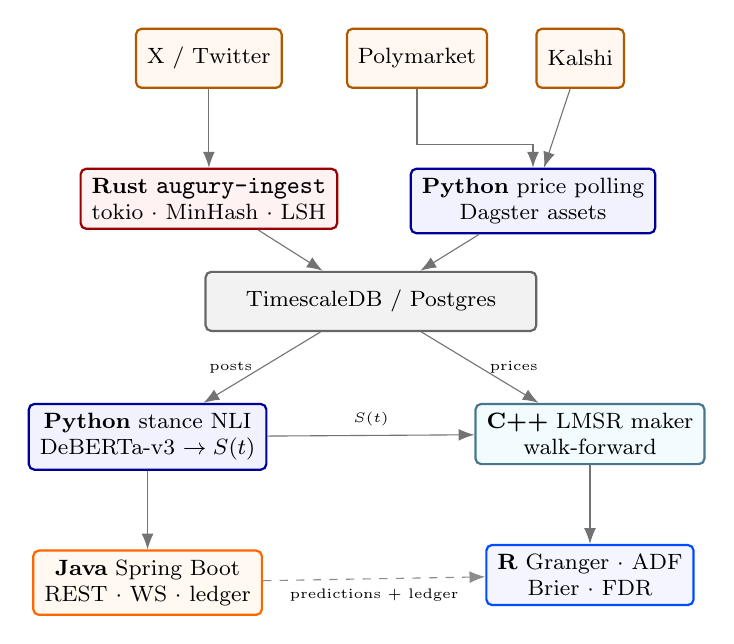
\begin{tikzpicture}[
  node distance=6mm,
  font=\footnotesize,
  box/.style={draw, rounded corners=2pt, minimum height=7.5mm, align=center,
              inner xsep=4pt, thick},
  src/.style={box, draw=orange!70!black, fill=orange!6},
  rs/.style={box, draw=red!60!black, fill=red!5},
  py/.style={box, draw=blue!60!black, fill=blue!5},
  cpp/.style={box, draw=cyan!50!black, fill=cyan!5},
  jv/.style={box, draw=orange!80!red, fill=orange!5},
  rl/.style={box, draw=blue!70!cyan, fill=blue!4},
  db/.style={box, draw=black!60, fill=black!5, minimum width=42mm},
  ar/.style={-{Latex[length=2mm]}, draw=black!55},
  dar/.style={-{Latex[length=2mm]}, draw=black!45, dashed}
]

\node[src] (x)    {X / Twitter};
\node[src, right=8mm of x] (poly) {Polymarket};
\node[src, right=6mm of poly] (kal) {Kalshi};

\node[rs, below=10mm of x] (rust) {\textbf{Rust} \code{augury-ingest}\\ tokio $\cdot$ MinHash $\cdot$ LSH};
\node[py, below=10mm of kal, xshift=-6mm] (pysig) {\textbf{Python} price polling\\ Dagster assets};

\node[db, below=9mm of $(rust)!0.5!(pysig)$] (db) {TimescaleDB / Postgres};

\node[py, below left=9mm and -8mm of db] (nlp) {\textbf{Python} stance NLI\\ DeBERTa-v3 $\to S(t)$};
\node[cpp, below right=9mm and -8mm of db] (cpp) {\textbf{C++} LMSR maker\\ walk-forward};

\node[jv, below=10mm of nlp] (java) {\textbf{Java} Spring Boot\\ REST $\cdot$ WS $\cdot$ ledger};
\node[rl, below=10mm of cpp] (r) {\textbf{R} Granger $\cdot$ ADF\\ Brier $\cdot$ FDR};

\draw[ar] (x) -- (rust);
\draw[ar] (poly) |- ([yshift=3mm]pysig.north) -- (pysig);
\draw[ar] (kal) -- (pysig);
\draw[ar] (rust) -- (db);
\draw[ar] (pysig) -- (db);
\draw[ar] (db) -- node[left, font=\tiny] {posts} (nlp);
\draw[ar] (db) -- node[right, font=\tiny] {prices} (cpp);
\draw[ar] (nlp) -- node[above, font=\tiny] {$S(t)$} (cpp);
\draw[ar] (nlp) -- (java);
\draw[ar] (cpp) -- (r);
\draw[dar] (java) -- node[below, font=\tiny] {predictions + ledger} (r);
\end{tikzpicture}
\caption[Service data flow across the five languages]{Data flow. Sources at the top, the durable record in the middle,
modelling and simulation below it, serving and econometrics at the bottom.
Every arrow crosses either the database or a schema-validated Redis channel;
no service holds a reference to another.}
\label{fig:arch}
\end{figure}

\begin{table}[htbp]
\centering
\caption[Services, responsibilities, and verification status]{Services, responsibilities, and verification status. Line counts cover
all git-tracked files of each type, test suites included.}
\label{tab:services}
\small
\begin{tabular}{@{}llrll@{}}
\toprule
Service & Language & LOC & Responsibility & Status \\
\midrule
\code{augury-signal}    & Python 3.12 & 7{,}545 & NLP, $S(t)$, orchestration & runs, 139 pass \\
\code{augury-ingest}    & Rust 1.97   & 2{,}469 & Streaming ingest, filter   & builds, 42 pass \\
\code{augury-engine}    & C++20       & 1{,}470 & LMSR, walk-forward         & builds, 26 pass \\
\code{augury-api}       & Java 25     & 1{,}222 & REST, WebSocket, ledger    & builds, 9 pass \\
\code{augury-analytics} & R 4.6       &   981   & Granger, Brier, reports    & runs, 55 pass \\
\midrule
Schema / migrations     & SQL, JSON   & 1{,}200 & Shared contracts           & migrations applied \\
\bottomrule
\end{tabular}
\end{table}

\subsection{Cross-service contracts}

Services never call each other directly. Two boundaries carry everything:

\textbf{TimescaleDB} is the durable record. A market is keyed everywhere as
\code{<venue>:<ticker>} (for example \code{kalshi:KXFEDDECISION-26SEP-C25}),
which is what keeps cross-venue joins unambiguous --- Kalshi tickers and
Polymarket condition ids share no namespace. Hypertable partitioning forces a
schema property worth noting: any unique constraint must include the
partitioning column, which is why \code{posts} is keyed on
$(\text{post\_id}, \text{market\_id}, \text{created\_at})$ rather than
\code{post\_id} alone. That is not merely a concession to Timescale; one post
can legitimately be evidence about two markets, and the compound key says so.

\textbf{Redis pub/sub} carries live updates on \code{augury.signal.*},
\code{augury.price.*}, and \code{augury.sim.*}. Payloads are validated against
JSON Schema \emph{at the publisher}. This is the only place the contract can be
enforced: the C++ and Java consumers are separately compiled and cannot be
type-checked against the Python publisher, so a schema check at the boundary is
the sole mechanism preventing silent drift. Redis is deliberately not a
dependency --- an outage degrades the live stream while ingestion, scoring, and
the REST API keep working off the database.

\begin{figure}[htbp]
\centering
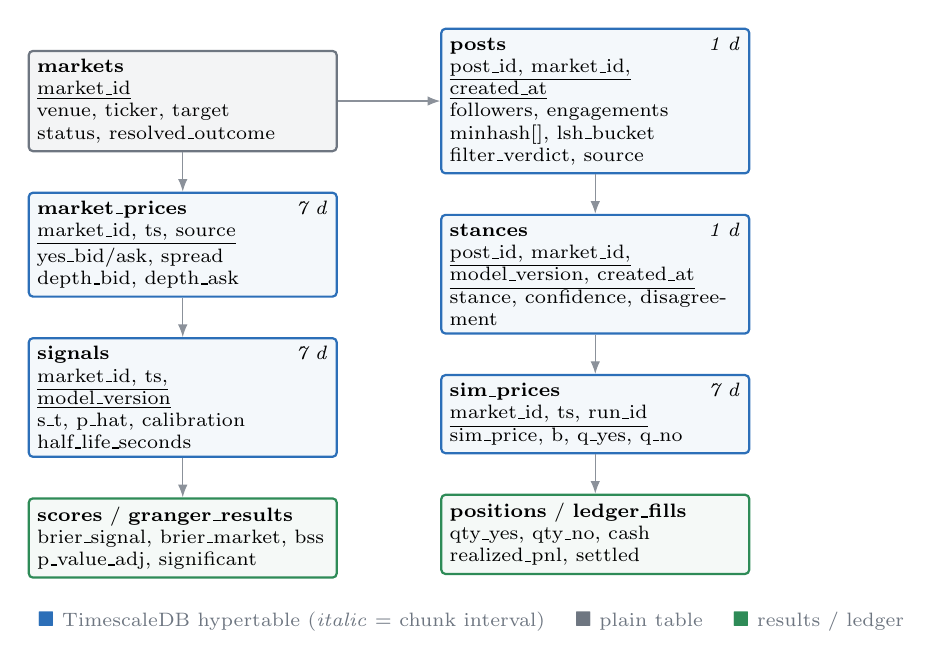
\begin{tikzpicture}[
  font=\scriptsize, node distance=4mm,
  tbl/.style={draw, thick, rounded corners=1.5pt, align=left, inner sep=3pt,
              text width=37mm},
  hyp/.style={tbl, draw=augBlue, fill=augBlue!5},
  rel/.style={tbl, draw=augGrey, fill=augGrey!8},
  led/.style={tbl, draw=augGreen, fill=augGreen!5},
  fk/.style={-{Latex[length=1.6mm]}, draw=augGrey!80},
]
\node[rel] (markets) {\textbf{markets}\\ \underline{market\_id}\\ venue, ticker, target\\ status, resolved\_outcome};
\node[hyp, right=13mm of markets] (posts) {\textbf{posts} \hfill \textit{1 d}\\ \underline{post\_id, market\_id,}\\ \underline{created\_at}\\ followers, engagements\\ minhash[], lsh\_bucket\\ filter\_verdict, source};
\node[hyp, below=5mm of posts] (stances) {\textbf{stances} \hfill \textit{1 d}\\ \underline{post\_id, market\_id,}\\ \underline{model\_version, created\_at}\\ stance, confidence, disagreement};
\node[hyp, below=5mm of markets] (prices) {\textbf{market\_prices} \hfill \textit{7 d}\\ \underline{market\_id, ts, source}\\ yes\_bid/ask, spread\\ depth\_bid, depth\_ask};
\node[hyp, below=5mm of prices] (signals) {\textbf{signals} \hfill \textit{7 d}\\ \underline{market\_id, ts,}\\ \underline{model\_version}\\ s\_t, p\_hat, calibration\\ half\_life\_seconds};
\node[hyp, below=5mm of stances] (sim) {\textbf{sim\_prices} \hfill \textit{7 d}\\ \underline{market\_id, ts, run\_id}\\ sim\_price, b, q\_yes, q\_no};
\node[led, below=5mm of signals] (scores) {\textbf{scores} / \textbf{granger\_results}\\ brier\_signal, brier\_market, bss\\ p\_value\_adj, significant};
\node[led, below=5mm of sim] (ledger) {\textbf{positions} / \textbf{ledger\_fills}\\ qty\_yes, qty\_no, cash\\ realized\_pnl, settled};

\draw[fk] (markets) -- (posts);
\draw[fk] (markets) -- (prices);
\draw[fk] (posts) -- (stances);
\draw[fk] (prices) -- (signals);
\draw[fk] (stances) -- (sim);
\draw[fk] (signals) -- (scores);
\draw[fk] (sim) -- (ledger);

\node[anchor=north west, align=left, augGrey, font=\scriptsize]
  at ([yshift=-3mm]scores.south west)
  {\textcolor{augBlue}{$\blacksquare$} TimescaleDB hypertable (\textit{italic} = chunk interval)
   \quad \textcolor{augGrey}{$\blacksquare$} plain table
   \quad \textcolor{augGreen}{$\blacksquare$} results / ledger};
\end{tikzpicture}
\caption[The shared TimescaleDB schema]{The shared schema. Underlined fields are the primary key. Every
hypertable's key includes its partitioning column --- a Timescale requirement,
but also a modelling one: \code{posts} is keyed on
$(\text{post\_id}, \text{market\_id}, \text{created\_at})$ because one post can
legitimately be evidence about two markets. \code{stances} is deliberately
separate from \code{posts} and keyed on \code{model\_version}, so re-scoring the
corpus with a new model cannot overwrite what an earlier model produced --- the
Brier comparison between versions depends on both surviving.}
\label{fig:schema}
\end{figure}

\begin{figure}[htbp]
\centering
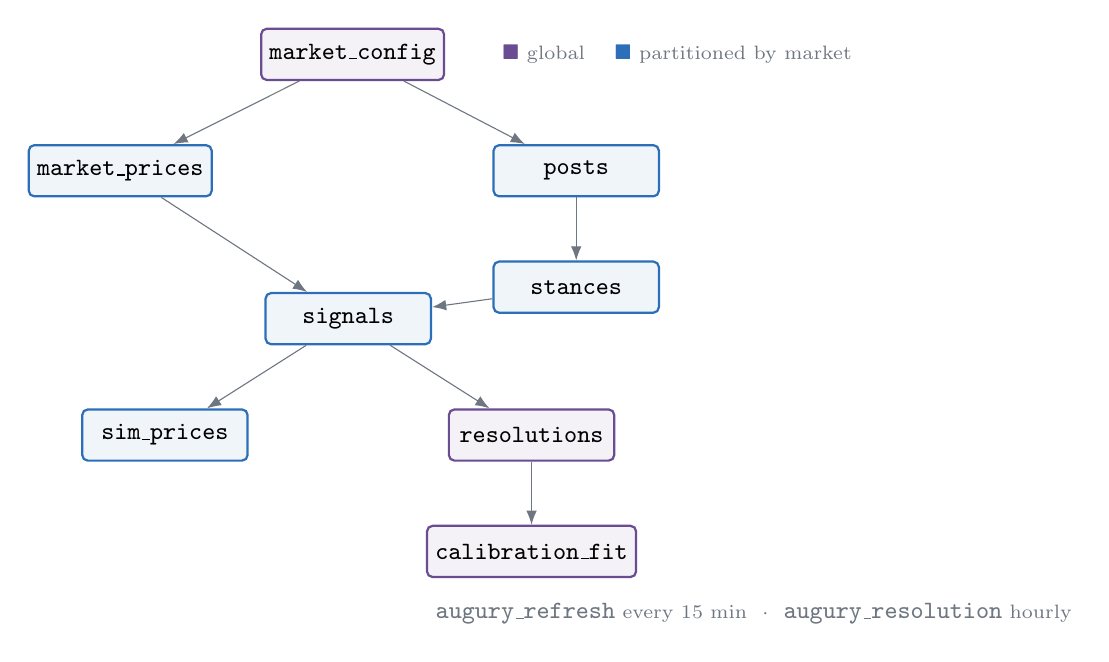
\begin{tikzpicture}[
  font=\footnotesize, node distance=5mm,
  ast/.style={draw, rounded corners=2pt, minimum height=6.5mm, minimum width=21mm,
              align=center, thick, inner xsep=3pt},
  part/.style={ast, draw=augBlue, fill=augBlue!7},
  glob/.style={ast, draw=augPurple, fill=augPurple!7},
  ar/.style={-{Latex[length=1.8mm]}, draw=augGrey},
]
\node[glob] (cfg) {\code{market\_config}};
\node[part, below left=8mm and 6mm of cfg] (prices) {\code{market\_prices}};
\node[part, below right=8mm and 6mm of cfg] (posts) {\code{posts}};
\node[part, below=8mm of posts] (stances) {\code{stances}};
\node[part, below=8mm of $(prices)!0.5!(stances)$, xshift=0mm] (signals) {\code{signals}};
\node[part, below left=8mm and 2mm of signals] (sim) {\code{sim\_prices}};
\node[glob, below right=8mm and 2mm of signals] (res) {\code{resolutions}};
\node[glob, below=8mm of res] (calfit) {\code{calibration\_fit}};

\draw[ar] (cfg) -- (prices);
\draw[ar] (cfg) -- (posts);
\draw[ar] (posts) -- (stances);
\draw[ar] (stances) -- (signals);
\draw[ar] (prices) -- (signals);
\draw[ar] (signals) -- (sim);
\draw[ar] (signals) -- (res);
\draw[ar] (res) -- (calfit);

\node[anchor=west, font=\scriptsize, augGrey] at ([xshift=6mm]cfg.east)
  {\textcolor{augPurple}{$\blacksquare$} global \quad \textcolor{augBlue}{$\blacksquare$} partitioned by market};
\node[anchor=north west, font=\scriptsize, augGrey, align=left]
  at ([yshift=-2mm]calfit.south west)
  {\code{augury\_refresh} every 15 min \ $\cdot$ \ \code{augury\_resolution} hourly};
\end{tikzpicture}
\caption[The Dagster asset graph]{The Dagster asset graph, as declared in
\code{pipeline/orchestrator.py}. The five blue assets are partitioned one
partition per tracked market, so a single venue outage fails one partition
rather than the run, and re-materialisation redoes only the market that failed.
Every asset writes through an idempotent upsert, which is what makes re-running
an overlapping window safe --- Dagster will happily retry a partition, and doing
so must not double-count posts in $S(t)$.}
\label{fig:dag}
\end{figure}

\section{The Social Signal $S(t)$}
\label{sec:signal}

Raw sentiment is the wrong quantity for a prediction market. What matters is a
post's \emph{stance} toward a specific claim, $\text{stance}_i \in [-1,1]$. The
aggregate signal at time $t$ is a weighted average under exponential decay:

\begin{equation}
S(t) \;=\;
\frac{\sum_{i=1}^{N(t)} w_i \, \text{stance}_i \, e^{-\lambda (t - t_i)}}
     {\sum_{i=1}^{N(t)} w_i \, e^{-\lambda (t - t_i)}},
\qquad
w_i = \ln(1 + f_i)\,(1 + e_i),
\qquad
\lambda = \frac{\ln 2}{t_{1/2}},
\label{eq:signal}
\end{equation}

with $f_i$ followers and $e_i$ engagements on post $i$. The logarithm on
followers is the usual reach compression; the linear factor on engagements
credits amplification.

\subsection{Log-space evaluation, and where float64 actually fails}

Both sums in Eq.~\ref{eq:signal} are evaluated in log space with the maximum
term factored out. Writing $\ell_i = \ln w_i - \lambda(t - t_i)$ and
$m = \max_i \ell_i$,

\begin{equation}
S(t) \;=\;
\frac{\sum_i \text{stance}_i \, e^{\ell_i - m}}{\sum_i e^{\ell_i - m}},
\label{eq:logspace}
\end{equation}

so the dominant term is $e^0 = 1$ and the common factor $e^{m}$ --- which may
be entirely unrepresentable --- cancels before it is ever formed.

The decay module's docstring motivates this by claiming that at a 30-minute
half-life a week-old post carries $e^{-233}$, ``which underflows to exactly zero
in float64.'' \textbf{That is not correct}, and the correction is worth stating
because it changes where the guard actually binds. IEEE-754 binary64 carries
subnormals down to $2^{-1074} \approx 4.94 \times 10^{-324}$, and because
$\exp$ rounds to nearest it survives until its result falls below half of that
--- so the first argument returning exactly zero is
$-1075 \ln 2 \approx -745.13$, verified by bisection. Concretely,
$e^{-233} = 7.14\times10^{-102}$, which is an entirely ordinary normalised
double. Table~\ref{tab:underflow} gives the real boundary.

\begin{table}[htbp]
\centering
\caption[Decay kernel magnitude by post age and half-life]{Decay kernel magnitude by post age and half-life. Underflow to exactly
zero begins at $\lambda \Delta t > 745.13$, or roughly 22.4 days at a 30-minute
half-life.}
\label{tab:underflow}
\small
\begin{tabular}{@{}llrl@{}}
\toprule
Half-life & Post age & $\lambda \Delta t$ & $e^{-\lambda \Delta t}$ \\
\midrule
6 h    & 7 d    & $19.41$  & $3.73 \times 10^{-9}$ \\
6 h    & 30 d   & $83.18$  & $7.52 \times 10^{-37}$ \\
30 min & 7 d    & $232.90$ & $7.14 \times 10^{-102}$ \\
30 min & 22.4 d & $745.27$ & $\mathbf{0}$ (underflow) \\
30 min & 30 d   & $998.13$ & $\mathbf{0}$ (underflow) \\
\bottomrule
\end{tabular}
\end{table}

\begin{figure}[htbp]
\centering
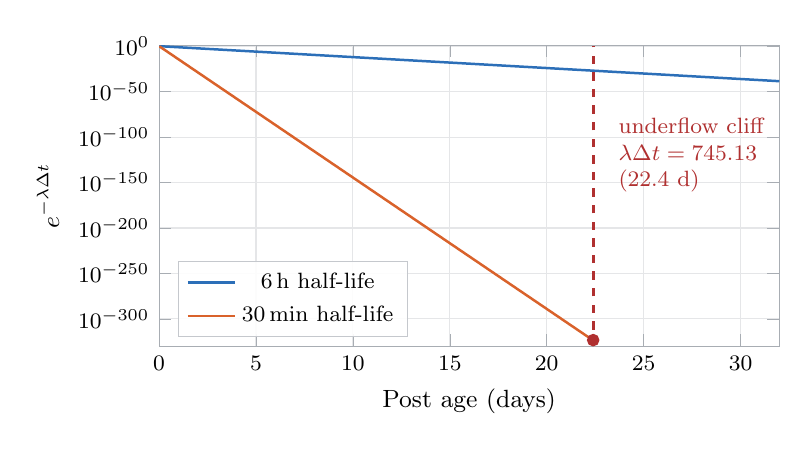
\begin{tikzpicture}
\begin{semilogyaxis}[
  augbase, height=5.4cm,
  xlabel={Post age (days)}, ylabel={$e^{-\lambda \Delta t}$},
  xmin=0, xmax=32, ymin=1e-330, ymax=5,
  ytick={1e0,1e-50,1e-100,1e-150,1e-200,1e-250,1e-300},
  legend pos=south west,
]
% 6-hour half-life
\addplot[augBlue, domain=0.01:32, samples=200]
  {exp(-0.693147/6 * x * 24)};
\addlegendentry{6\,h half-life}
% 30-minute half-life
\addplot[augOrange, domain=0.01:22.396, samples=200]
  {exp(-0.693147/0.5 * x * 24)};
\addlegendentry{30\,min half-life}
% the cliff
\addplot[augRed, dashed, line width=1pt] coordinates {(22.396,1e-330) (22.396,5)};
\addplot[augRed, only marks, mark=*, mark size=1.8pt] coordinates {(22.396,4.94e-324)};
\node[font=\footnotesize, augRed, anchor=west, align=left]
  at (axis cs:23.2,1e-120) {underflow cliff\\ $\lambda\Delta t = 745.13$\\ (22.4 d)};
\end{semilogyaxis}
\end{tikzpicture}
\caption[The decay kernel and the float64 underflow cliff]{The decay kernel over 32 days. At a 6-hour half-life nothing comes close
to the boundary. At the 30-minute half-life the adaptive path can reach, the
kernel falls off the representable range entirely at 22.4 days --- the orange
curve simply stops, because beyond that point every term in both sums of
Eq.~\ref{eq:signal} is exactly zero and the naive ratio is $0/0$. The widely
quoted $e^{-233}$ at one week sits at $10^{-102}$, nowhere near the cliff.}
\label{fig:underflow}
\end{figure}

The guard is still necessary, and the shipped test data proves it. The golden
vector named \code{extreme\_age} evaluates a 30-day-old post at a 30-minute
half-life, giving $\lambda \Delta t = 998$. Its recorded expectations are
$s_t = 0.5$ --- the stance of the only post present, which
Eq.~\ref{eq:logspace} recovers correctly --- alongside
$\texttt{weight\_sum} = 0.0$ \emph{exactly}. That second field is the underflow
itself, pinned as a fact in the test data: the absolute weight has vanished
while the ratio remains well defined. A naive implementation would compute
$0/0$ here. What the code does is right; only the stated threshold was off, by a
factor of three in the conservative direction, and a reader calibrating a
shorter half-life from the documented figure would have over-estimated the
danger zone.

\subsection{Two degenerate cases handled rather than papered over}

A zero-follower account gets $\ln(1) = 0$ and therefore contributes
\emph{nothing}, no matter how much engagement the post drew. That is what
Eq.~\ref{eq:signal} says, so it is what the implementation does --- but it means
a window containing only zero-follower posts has no defined signal. In that
case, and when the window is empty, \code{compute\_signal} returns \code{None}
rather than $0.0$.

The distinction is load-bearing. Zero is a real, neutral signal value. Returning
it for ``nobody has said anything'' would tell the downstream LMSR that the
crowd is balanced when in fact the crowd is silent, and the market maker would
then trade on a claim nobody made. Every consumer is required to propagate the
absence rather than substitute a default.

Separately, posts timestamped after the evaluation instant are excluded
unconditionally. This is the single cheapest place to introduce lookahead into a
backtest, and it is precisely the bug that makes a lead--lag result look
spectacular and be worthless.

\subsection{Adaptive half-lives}

A fixed six-hour half-life means that during an FOMC statement or a debate,
posts from before the news still dominate the average. The effective half-life
is therefore shortened in proportion to how unusual the current window is, under
two independent triggers, whichever is stronger:

\begin{equation}
t_{1/2}^{\text{eff}} = \max\!\left(t_{\min},\;
\frac{t_{1/2}}{\max\big(1,\, \tfrac{n_{\text{recent}}}{\kappa \, r_{\text{base}}},\,
\tfrac{|\Delta p|}{\theta}\big)}\right),
\end{equation}

with $\kappa$ the volume-surge multiple (default 3), $\theta$ the price-move
threshold (default 0.05), and $t_{\min}$ a configurable floor (default 30
minutes). Below both triggers the factor is exactly 1, so a quiet market keeps
its baseline half-life bit-for-bit.

Two details matter. The baseline rate $r_{\text{base}}$ is the \emph{median}
hourly post count over a trailing 24 hours, not the mean: one viral hour would
otherwise raise the baseline enough to mask the next surge, which is exactly
when the shortened half-life is wanted. And that median is floored at one post
per hour, because most tracked markets are quiet most of the time and a median
of zero would make the surge ratio undefined --- silently disabling the trigger
in the case where it is most informative, a quiet market that suddenly receives
thirty posts.

\begin{figure}[htbp]
\centering
\begin{tikzpicture}
\begin{axis}[
  augbase, width=0.72\textwidth, height=5.6cm,
  xlabel={Posts in trailing hour (baseline $r_{\text{base}} = 5$/h)},
  ylabel={$|\Delta p|$ over trailing hour},
  view={0}{90},
  colormap/viridis,
  colorbar,
  colorbar style={
    title={\footnotesize $t_{1/2}^{\text{eff}}$ (h)},
    ytick={0.5,1.5,3,4.5,6},
    tick label style={font=\footnotesize}
  },
  xmin=0, xmax=60, ymin=0, ymax=0.25,
  point meta min=0.5, point meta max=6,
]
\addplot3[surf, shader=interp, mesh/ordering=x varies, mesh/cols=31]
  table[x=posts, y=move, z=half_life_h, col sep=comma] {data/halflife_grid.csv};
% trigger thresholds
\addplot3[augRed, dashed, line width=0.9pt] coordinates {(0,0.05,10) (60,0.05,10)};
\addplot3[augRed, dashed, line width=0.9pt] coordinates {(15,0,10) (15,0.25,10)};
\node[annot, anchor=south west] at (axis cs:0.8,0.005,10) {baseline plateau: 6.00\,h};
\node[annot, text=augRed, anchor=south west] at (axis cs:34,0.052,10) {$\theta = 0.05$};
\node[annot, text=augRed, anchor=south west] at (axis cs:16,0.20,10) {$\kappa r_{\text{base}} = 15$};
\end{axis}
\end{tikzpicture}
\caption[Effective half-life under the two adaptive triggers]{Effective half-life as a function of the two adaptive triggers,
evaluated by calling \code{effective\_half\_life} over a grid. Inside both
thresholds (lower-left block) the factor is exactly $1$ and the baseline 6-hour
half-life is preserved bit-for-bit. Either trigger alone shortens it; the
surface saturates at the configured floor $t_{\min} = 30$ minutes. The two
mechanisms are combined by $\max$, not by summation, so a market that is both
busy and moving is not double-counted.}
\label{fig:halflife}
\end{figure}

Because the half-life varies, it is recorded per signal point in the
\code{signals} table rather than assumed constant. A series whose decay
parameter moved is not comparable to one where it stayed fixed, and the column
is what makes that distinction recoverable after the fact.

\section{Target-Conditioned Stance}
\label{sec:stance}

Standard sentiment analysis fails on prediction-market phrasing in a specific
and systematic way. ``Candidate X drops out'' is negative \emph{text sentiment}
and strongly \emph{bullish stance} toward ``Will Candidate Y win?''. A lexicon
scores the words and gets the sign backwards.

Augury encodes each post and the market's target claim as a natural-language
inference sentence pair --- premise $=$ post, hypothesis $=$ claim --- and
derives

\begin{equation}
\text{stance} = P(\text{entail}) - P(\text{contradict}),
\qquad
\text{confidence} = 1 - P(\text{neutral}).
\end{equation}

This mapping has a property worth stating: a post the model finds neutral
receives a stance near zero \emph{and} a low confidence, so it neither pushes
the signal nor claims to be informative. The two quantities degrade together,
which is what one wants from an uncertainty estimate.

Consequently every tracked market carries a declarative \code{target} in
\code{config/markets.yaml} --- a claim, never a question, because entailment
against an interrogative is ill-defined and the outputs drift toward neutral.
The market titled ``Will the Federal Reserve cut rates by 25bps at their
September 2026 meeting?'' carries the target ``The Federal Reserve will cut
interest rates by 25 basis points at its September 2026 meeting.''

Three implementation choices are worth recording. First, NLI label names vary
across checkpoints (\code{ENTAILMENT}, \code{entailment}, \code{LABEL\_0}), so
the model's own \code{id2label} map is inspected by regular expression rather
than assumed, and a checkpoint whose entailment and contradiction indices cannot
be identified raises instead of guessing. Second, weight loading is lazy, so
constructing the model is free and the several hundred megabytes are pulled only
when something is actually scored --- which keeps the test suite and the
\code{markets} subcommand from downloading a model they will never use. Third,
the checkpoint default points at an NLI-tuned model, because plain
\code{deberta-v3-base} is a pretrained encoder with a \emph{randomly initialised}
classification head: it has no concept of entailment, and using it directly
would produce confident noise rather than an error.

A VADER lexicon model is retained as the ensemble's second opinion. It cannot,
by construction, condition on the target, so it is not a competitor --- it is a
disagreement detector. The per-post quantity
$|\text{stance}_{\text{NLI}} - \text{stance}_{\text{VADER}}|$ is stored as a
data-quality flag, on the reasoning that a post the target-conditioned model
reads as bullish and the lexicon reads as bearish is either the exact case the
NLI framing exists to handle, or a post ambiguous enough to distrust.

\section{Ingestion and Near-Duplicate Filtering}
\label{sec:ingest}

A spam ring posting the same claim from fifty accounts with rotated links and
minor edits moves $S(t)$ as much as fifty genuine opinions. Exact hashing catches
none of it.

\subsection{MinHash and LSH}

For a random permutation of the shingle universe, the probability that two sets
share a minimum element is exactly their Jaccard similarity; averaging that
indicator over $H$ independent permutations gives an unbiased estimate with
standard error $\approx 1/\sqrt{H}$. The implementation uses word trigrams over
normalised text, $H = 128$ permutations drawn from the universal family
$h_i(x) = (a_i x + b_i) \bmod p$ with $p = 2^{61}-1$, and a deterministic
splitmix64 seed --- deterministic because signatures are persisted to
\code{BIGINT[]} columns and compared against posts hashed by a later process run
on a different machine.

Normalisation strips URLs, mentions, cashtags, and hashtags. This is the correct
direction for an adversarial filter: a spam ring rotates its links and handles
while reusing the body, so \emph{keeping} those tokens would make otherwise
identical posts look distinct.

\begin{algorithm}[t]
\caption{Streaming near-duplicate check against a bounded window}
\label{alg:dup}
\begin{algorithmic}[1]
\Require post $(id, \text{text})$, window $W$ (capacity $C$), threshold $\tau$
\Ensure verdict, and the signature to persist
\State $\sigma \gets \textsc{MinHash}(\text{text})$
\If{$\sigma = \bot$} \Comment{no shingles: URLs and handles only}
  \State \Return $(\textsc{Unique}, \bot)$ \Comment{cannot be a duplicate of anything}
\EndIf
\State $B \gets \textsc{Buckets}(\sigma)$ \Comment{one LSH key per band}
\State $best \gets \bot$
\For{$s \in W$}
  \If{$B \cap s.\text{buckets} = \emptyset$} \textbf{continue} \Comment{LSH pre-filter}
  \EndIf
  \State $j \gets \textsc{Similarity}(\sigma, s.\sigma)$ \Comment{exact signature agreement}
  \If{$j \ge \tau$ \textbf{and} ($best = \bot$ \textbf{or} $j > best.j$)}
    \State $best \gets (s, j)$
  \EndIf
\EndFor
\If{$|W| = C$} \State evict oldest from $W$ \EndIf
\State push $(id, \sigma, B)$ onto $W$ \Comment{duplicates are remembered too}
\State \Return $(best = \bot \;?\; \textsc{Unique} : \textsc{Duplicate}(best), \sigma)$
\end{algorithmic}
\end{algorithm}

Algorithm~\ref{alg:dup} has two properties chosen deliberately. Duplicates are
pushed onto the window along with originals, so a ring posting twenty variants
matches against the whole cluster rather than only its first member. And the
window is bounded --- an unbounded index grows without limit over a long ingest
run, and comparing against month-old posts is not useful anyway, since the same
phrasing recurring next week is a separate event rather than a duplicate. The
bound is what makes this a \emph{streaming} filter.

\subsection{The banding is mistuned}

Splitting an $H$-permutation signature into $b$ bands of $r$ rows makes two
documents with Jaccard similarity $s$ collide in at least one band with
probability

\begin{equation}
P_{\text{compare}}(s) \;=\; 1 - (1 - s^{r})^{b}.
\label{eq:scurve}
\end{equation}

The shipped configuration is $H = 128$, $b = 8$, $r = 16$, with a duplicate
threshold of $\tau = 0.80$. A source comment states that this ``crosses 50\%
around Jaccard 0.80.'' It does not. Solving Eq.~\ref{eq:scurve} numerically,
the 50\% point for $(b,r) = (8,16)$ is $s = 0.856$, and at the declared
threshold $\tau = 0.80$ the probability that a genuine duplicate pair is even
\emph{compared} is $20.4\%$ (Table~\ref{tab:lsh}, Figure~\ref{fig:scurve}).
Roughly four in five true duplicates at threshold are never examined.

\begin{table}[htbp]
\centering
\caption[LSH retrieval probability by Jaccard similarity]{Probability that a pair with Jaccard similarity $s$ is retrieved for
comparison. The shipped configuration's steep region sits to the \emph{right}
of the $\tau = 0.80$ decision threshold, which is the wrong side.}
\label{tab:lsh}
\small
\begin{tabular}{@{}lrrrrrrr@{}}
\toprule
$s$ & $0.60$ & $0.70$ & $0.75$ & $\mathbf{0.80}$ & $0.85$ & $0.90$ & $0.95$ \\
\midrule
shipped $(b{=}8, r{=}16)$   & 0.002 & 0.026 & 0.077 & \textbf{0.204} & 0.461 & 0.806 & 0.990 \\
proposed $(b{=}16, r{=}8)$  & 0.237 & 0.613 & 0.815 & \textbf{0.947} & 0.994 & 1.000 & 1.000 \\
\bottomrule
\end{tabular}
\end{table}

\begin{figure}[htbp]
\centering
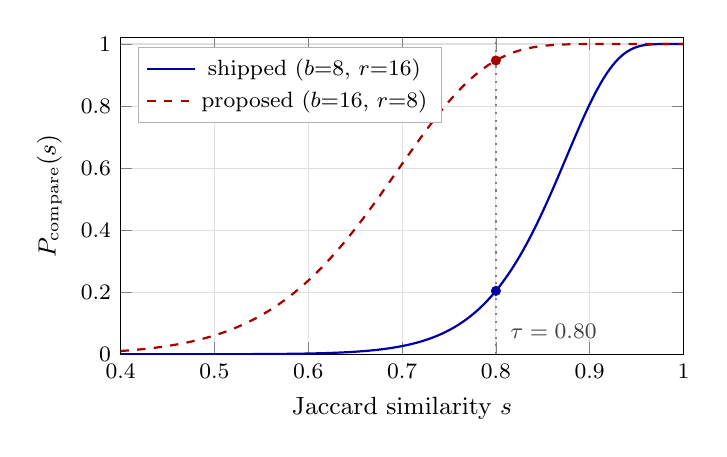
\begin{tikzpicture}
\begin{axis}[
  width=0.72\textwidth, height=5.6cm,
  xlabel={Jaccard similarity $s$},
  ylabel={$P_{\text{compare}}(s)$},
  xmin=0.4, xmax=1.0, ymin=0, ymax=1.02,
  grid=major, grid style={black!12},
  legend pos=north west, legend style={font=\footnotesize, draw=black!30},
  tick label style={font=\footnotesize},
  label style={font=\small}
]
\addplot[thick, blue!65!black, domain=0.4:1.0, samples=200]
  {1 - (1 - x^16)^8};
\addlegendentry{shipped $(b{=}8,\,r{=}16)$}
\addplot[thick, red!65!black, dashed, domain=0.4:1.0, samples=200]
  {1 - (1 - x^8)^16};
\addlegendentry{proposed $(b{=}16,\,r{=}8)$}
\addplot[gray, dotted, thick] coordinates {(0.8,0) (0.8,1.02)};
\node[font=\footnotesize, gray!50!black, anchor=south west] at (axis cs:0.805,0.02) {$\tau = 0.80$};
\addplot[only marks, mark=*, mark size=1.6pt, blue!65!black] coordinates {(0.8,0.2042)};
\addplot[only marks, mark=*, mark size=1.6pt, red!65!black] coordinates {(0.8,0.9470)};
\end{axis}
\end{tikzpicture}
\caption[LSH retrieval probability against the duplicate threshold]{LSH retrieval probability. The decision threshold is $\tau = 0.80$;
the shipped banding retrieves only $20.4\%$ of true duplicates there.}
\label{fig:scurve}
\end{figure}

The fix follows from an asymmetry in the costs. LSH here is purely a
\emph{pre-filter}: every retrieved candidate is then subjected to an exact
signature comparison against $\tau$, so a false positive from banding costs one
128-element integer comparison and nothing else, while a false negative is a
duplicate that silently enters $S(t)$ as an independent opinion. The banding
should therefore be tuned so its steep region sits to the \emph{left} of the
decision threshold. Repartitioning the same 128 permutations as $b = 16$ bands
of $r = 8$ rows moves the 50\% point to $s = 0.674$ and lifts retrieval at
$\tau = 0.80$ to $94.7\%$, at the price of examining $23.7\%$ of pairs at
$s = 0.60$ --- all of which the exact check then rejects. No additional storage
or hashing is required; it is a repartitioning of an existing signature.

\begin{figure}[htbp]
\centering
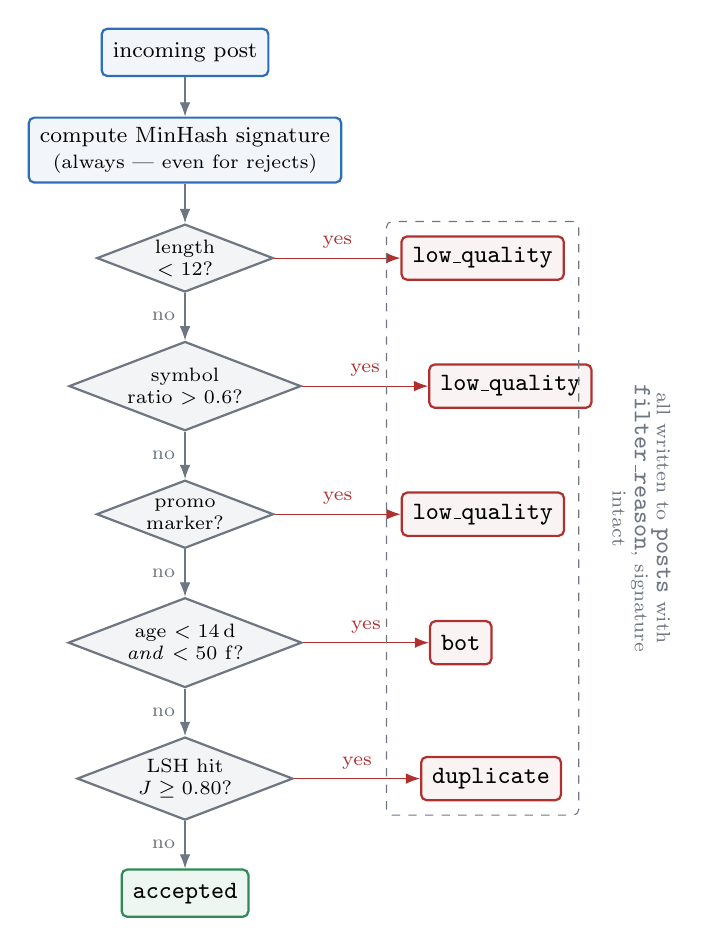
\begin{tikzpicture}[
  font=\footnotesize, node distance=4mm,
  fstep/.style={draw, thick, rounded corners=2pt, minimum height=6mm, align=center,
               inner xsep=4pt, draw=augBlue, fill=augBlue!6},
  dec/.style={draw, thick, diamond, aspect=2.6, inner sep=1pt, align=center,
              draw=augGrey, fill=augGrey!8, font=\scriptsize},
  rej/.style={draw, thick, rounded corners=2pt, align=center, inner xsep=4pt,
              minimum height=5.5mm, draw=augRed, fill=augRed!6, font=\scriptsize},
  acc/.style={fstep, draw=augGreen, fill=augGreen!8},
  ar/.style={-{Latex[length=1.8mm]}, draw=augGrey},
]
\node[fstep] (in) {incoming post};
\node[fstep, below=5mm of in] (sig) {compute MinHash signature\\ \scriptsize(always --- even for rejects)};
\node[dec, below=5mm of sig] (len) {length\\ $<12$?};
\node[dec, below=6mm of len] (sym) {symbol\\ ratio $>0.6$?};
\node[dec, below=6mm of sym] (spam) {promo\\ marker?};
\node[dec, below=6mm of spam] (bot) {age $<14$\,d\\ \emph{and} $<50$ f?};
\node[dec, below=6mm of bot] (dup) {LSH hit\\ $J \ge 0.80$?};
\node[acc, below=6mm of dup] (ok) {\code{accepted}};

\node[rej, right=16mm of len] (r1) {\code{low\_quality}};
\node[rej, right=16mm of sym] (r2) {\code{low\_quality}};
\node[rej, right=16mm of spam] (r3) {\code{low\_quality}};
\node[rej, right=16mm of bot] (r4) {\code{bot}};
\node[rej, right=16mm of dup] (r5) {\code{duplicate}};

\draw[ar] (in) -- (sig);
\draw[ar] (sig) -- (len);
\foreach \a/\b in {len/sym, sym/spam, spam/bot, bot/dup, dup/ok}
  \draw[ar] (\a) -- node[left, font=\scriptsize, augGrey] {no} (\b);
\foreach \d/\r in {len/r1, sym/r2, spam/r3, bot/r4, dup/r5}
  \draw[ar, augRed] (\d) -- node[above, font=\scriptsize, augRed] {yes} (\r);

\node[draw, dashed, augGrey, rounded corners=2pt, fit=(r1)(r5), inner sep=5pt] (box) {};
\node[anchor=west, align=left, font=\scriptsize, augGrey] at ([xshift=3mm]box.east)
  {\rotatebox{-90}{\parbox{34mm}{\centering all written to \code{posts} with\\ \code{filter\_reason}, signature intact}}};
\end{tikzpicture}
\caption[The bot and near-duplicate filter decision order]{The filter's decision order. Cheap field checks precede the MinHash
comparison so obvious junk never reaches the expensive path --- but the
signature is computed \emph{first}, unconditionally, so a rejected post can
still be compared against later arrivals. No branch discards a post: every
verdict is persisted with its reason, which is the only thing that makes the
filter's own precision measurable after the fact. Thresholds shown are the
shipped defaults.}
\label{fig:filter}
\end{figure}

\subsection{Rejects are stored, not dropped}

Rejected posts are written to the database with their verdict
(\code{duplicate}, \code{bot}, \code{low\_quality}) and a human-readable reason,
alongside their MinHash signature. Without the rejects there is no way to
measure how often the filter is wrong, and a filter nobody can audit is a filter
nobody should trust. The signal query reads through a partial index
(\code{WHERE filter\_verdict = 'accepted'}), so retaining the rejects costs
storage but not query time.

The heuristic thresholds are deliberately loose --- account age under 14 days
\emph{and} fewer than 50 followers, text under 12 characters, symbol ratio above
0.6, a small promotional-marker list --- on the reasoning that wrongly dropping
a real opinion silently biases the signal, whereas letting a little junk through
adds noise that the follower weighting already discounts. A young account with a
real audience is a person, not a ring, and passes.

\subsection{The read budget}

X charges roughly \$0.005 per post read, so the budget is the only thing between
a polling loop and a real bill. Two properties are non-negotiable. It must
survive restarts, because an in-process counter resets on every crash and a
crash loop then becomes unbounded spending; the counter therefore lives in a
\code{read\_budget} table keyed by (UTC day, service). And it must be reserved
\emph{before} the request goes out, because a request that times out after the
server has already metered it would otherwise slip through unbilled.

The reservation is a single statement so that two concurrent workers cannot both
observe headroom and both spend it:

\begin{lstlisting}
INSERT INTO read_budget (day, service, reads_used)
SELECT CURRENT_DATE, $1, $2 WHERE $2 <= $3
ON CONFLICT (day, service) DO UPDATE
    SET reads_used = read_budget.reads_used + EXCLUDED.reads_used
    WHERE read_budget.reads_used + EXCLUDED.reads_used <= $3
RETURNING reads_used
\end{lstlisting}

Both guards are required, and the reason is a defect this codebase shipped with
before review. On the first request of a UTC day there is no conflicting row, so
\code{ON CONFLICT} never fires --- and the natural \code{INSERT ... VALUES} form
would happily insert a single reservation larger than the entire daily budget.
The \code{WHERE} clause on the \code{SELECT} closes that hole; the
\code{ON CONFLICT} guard covers every subsequent request. Unused reservations
are refunded after the response arrives, without which the effective ceiling
would collapse from the number of \emph{reads} to the number of \emph{requests}.

\begin{figure}[htbp]
\centering
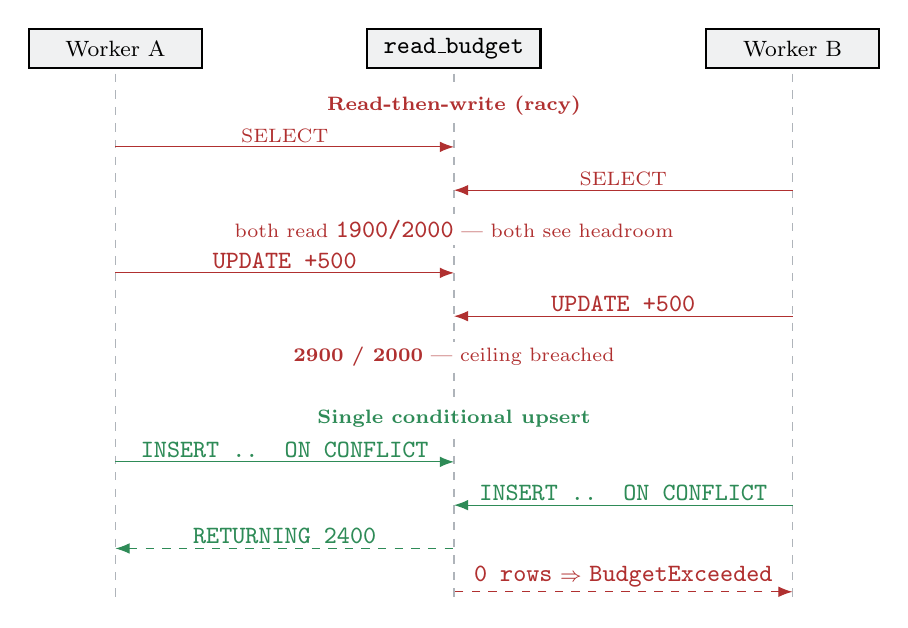
\begin{tikzpicture}[font=\footnotesize, >={Latex[length=1.8mm]},
  msg/.style={font=\scriptsize, inner sep=1.5pt},
  note/.style={font=\scriptsize, fill=white, inner sep=2pt, align=center}]
\foreach \x/\name in {0/{Worker A}, 4.3/{\code{read\_budget}}, 8.6/{Worker B}} {
  \node[draw, thick, fill=augGrey!10, minimum width=22mm, minimum height=5mm] at (\x,0) {\name};
  \draw[augGrey!55, dashed] (\x,-0.32) -- (\x,-7.0);
}
% ---- phase 1: racy
\node[note, text=augRed, font=\scriptsize\bfseries] at (4.3,-0.72) {Read-then-write (racy)};
\draw[->, augRed] (0,-1.25)   -- node[msg, above] {SELECT} (4.3,-1.25);
\draw[->, augRed] (8.6,-1.80) -- node[msg, above] {SELECT} (4.3,-1.80);
\node[note, text=augRed] at (4.3,-2.30) {both read \code{1900/2000} --- both see headroom};
\draw[->, augRed] (0,-2.85)   -- node[msg, above] {\code{UPDATE +500}} (4.3,-2.85);
\draw[->, augRed] (8.6,-3.40) -- node[msg, above] {\code{UPDATE +500}} (4.3,-3.40);
\node[note, text=augRed] at (4.3,-3.92) {\textbf{2900 / 2000} --- ceiling breached};
% ---- phase 2: atomic
\node[note, text=augGreen, font=\scriptsize\bfseries] at (4.3,-4.70) {Single conditional upsert};
\draw[->, augGreen] (0,-5.25)   -- node[msg, above] {\code{INSERT .. ON CONFLICT}} (4.3,-5.25);
\draw[->, augGreen] (8.6,-5.80) -- node[msg, above] {\code{INSERT .. ON CONFLICT}} (4.3,-5.80);
\draw[<-, augGreen, dashed] (0,-6.35) -- node[msg, above] {\code{RETURNING 2400}} (4.3,-6.35);
\draw[<-, augRed, dashed] (8.6,-6.90) -- node[msg, above] {\code{0 rows} $\Rightarrow$ \code{BudgetExceeded}} (4.3,-6.90);
\end{tikzpicture}
\caption[Why the read-budget reservation must be one statement]{Why the reservation must be one statement. The \code{WHERE} clause
lives inside the upsert, so the check and the increment are a single atomic
operation and the loser of the race is told it lost. A read followed by a write
lets both workers observe the same headroom and both spend it --- at
\$0.005 a read, silently.}
\label{fig:budget}
\end{figure}

Finally, anything derived from replayed fixtures carries \code{source='fixture'}
into the database, so a number computed from replayed data can never later be
mistaken for a real measurement.

\section{The LMSR Synthetic Market}
\label{sec:lmsr}

Hanson's Logarithmic Market Scoring Rule defines a cost function and the price
vector implied by its gradient:

\begin{equation}
C(\mathbf{q}) = b \ln\!\Big(\sum_{j=1}^{K} e^{q_j/b}\Big),
\qquad
p_k(\mathbf{q}) = \frac{e^{q_k/b}}{\sum_{j} e^{q_j/b}},
\qquad
\text{cost}(\mathbf{q} \to \mathbf{q}+d\mathbf{q}) = C(\mathbf{q}+d\mathbf{q}) - C(\mathbf{q}).
\end{equation}

For a binary market the structure collapses to a sigmoid,
$p_{\text{yes}} = \sigma\!\big((q_{\text{yes}} - q_{\text{no}})/b\big)$, hence

\begin{equation}
\operatorname{logit}(p_{\text{yes}}) = \frac{q_{\text{yes}} - q_{\text{no}}}{b},
\label{eq:logitid}
\end{equation}

so buying $n$ YES shares moves $\operatorname{logit}(p)$ by exactly $n/b$. That
linearity is what makes $b$ interpretable as liquidity and is the basis of
everything below.

\subsection{Calibrating $b$ from observed depth}

The liquidity parameter controls both the market maker's worst-case subsidy
$b \ln K$ and how far a single trade moves the price. Chosen arbitrarily, the
synthetic market either barely reacts to the signal or whipsaws on every post,
and tuning it until the output looks convincing is exactly the degree of freedom
that makes a simulation unfalsifiable. It is therefore derived.

In a real book, consuming the size resting between the bid and the ask walks the
price across the quoted range. By Eq.~\ref{eq:logitid}, moving the synthetic
price that same distance costs
$b\,\big(\operatorname{logit}(\text{ask}) - \operatorname{logit}(\text{bid})\big)$
shares. Setting the two equal:

\begin{equation}
b = \frac{\text{depth}}{\operatorname{logit}(\text{ask}) - \operatorname{logit}(\text{bid})}.
\label{eq:calib}
\end{equation}

Recalibrating $b$ between trades deliberately holds the current price fixed: by
Eq.~\ref{eq:logitid}, preserving $p$ under a change of $b$ means rescaling the
share imbalance by the same ratio. This is a modelling commitment, not an
implementation convenience --- a liquidity update is not new information about
the outcome, and letting it move the price would inject signal that nobody
traded on.

\subsection{Real books are severely lopsided}

Equation~\ref{eq:calib} leaves one choice open: which side's depth. On a
symmetric book it does not matter. Real prediction-market books are not
symmetric. Table~\ref{tab:depth} applies Eq.~\ref{eq:calib} to a live Kalshi
snapshot of \code{KXFEDDECISION-26SEP-C25} taken during the run in
Section~\ref{sec:worked}.

\begin{table}[htbp]
\centering
\caption[Depth calibration on a live Kalshi book]{Depth calibration on a live Kalshi book: bid $0.03 \times 93$, ask
$0.04 \times 67{,}296$. The logit width is $0.2980$. The choice of side changes
$b$ by a factor of $723$.}
\label{tab:depth}
\small
\begin{tabular}{@{}lrrr@{}}
\toprule
Side used & Depth (shares) & $b$ & Worst-case subsidy $b \ln 2$ \\
\midrule
bid only  & $93.0$      & $312$        & \$216 \\
mean      & $33{,}694.6$ & $113{,}052$  & \$78{,}362 \\
ask only  & $67{,}296.1$ & $225{,}792$  & \$156{,}507 \\
\bottomrule
\end{tabular}
\end{table}

\begin{figure}[htbp]
\centering
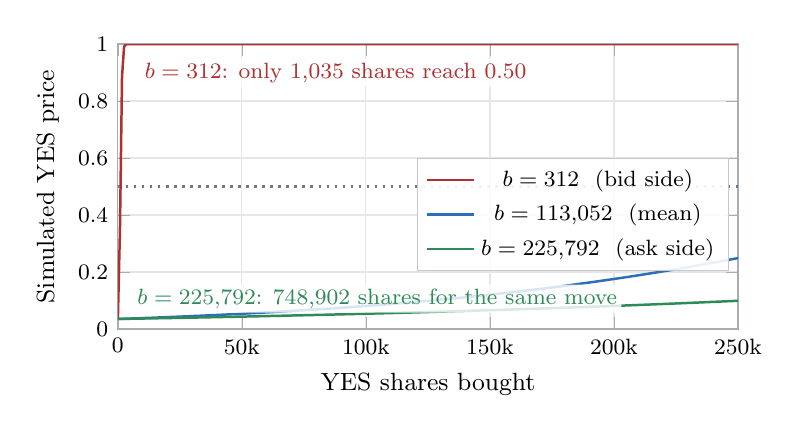
\begin{tikzpicture}
\begin{axis}[
  augbase, height=5.2cm,
  xlabel={YES shares bought}, ylabel={Simulated YES price},
  xmin=0, xmax=250000, ymin=0, ymax=1,
  scaled x ticks=false,
  xtick={0,50000,100000,150000,200000,250000},
  xticklabels={0,50k,100k,150k,200k,250k},
  legend style={at={(0.985,0.60)}, anchor=north east},
]
% p = sigmoid(logit(0.035) + n/b), anchored at the observed mid
\addplot[augRed, domain=0:250000, samples=300]
  {1/(1+exp(-(ln(0.035/0.965) + x/312)))};
\addlegendentry{$b = 312$ \ (bid side)}
\addplot[augBlue, domain=0:250000, samples=300]
  {1/(1+exp(-(ln(0.035/0.965) + x/113052)))};
\addlegendentry{$b = 113{,}052$ \ (mean)}
\addplot[augGreen, domain=0:250000, samples=300]
  {1/(1+exp(-(ln(0.035/0.965) + x/225792)))};
\addlegendentry{$b = 225{,}792$ \ (ask side)}
\addplot[augGrey, dotted, line width=0.9pt] coordinates {(0,0.5) (250000,0.5)};
\node[annot, text=augRed, anchor=west] at (axis cs:9000,0.90)
  {$b=312$: only $1{,}035$ shares reach $0.50$};
\node[annot, text=augGreen, anchor=south west] at (axis cs:6000,0.055)
  {$b=225{,}792$: $748{,}902$ shares for the same move};
\end{axis}
\end{tikzpicture}
\caption[LMSR price impact under the three calibrations of $b$]{What the $723\times$ ambiguity actually costs. Each curve is the same
LMSR anchored at the observed mid of $0.035$, differing only in which side of the
book $b$ was calibrated from. On the bid-side calibration a retail-sized order
moves the synthetic market across its whole range; on the ask-side calibration
no realistic trade moves it at all. The simulation's entire character is
determined by a choice the data does not settle.}
\label{fig:bimpact}
\end{figure}

A $723\times$ spread in the single parameter that governs how responsive the
simulated market is cannot be resolved by picking a default and moving on. The
default here averages both sides, which is symmetric but not obviously correct;
the honest reading of Table~\ref{tab:depth} is that on a deeply
out-of-the-money market the ask side is thick because nobody wants the position
at all, and the bid side is thin for the same reason, so neither number is
measuring ``liquidity'' in the sense the model assumes. This is recorded as an
open question rather than a solved one, and \code{side} is a first-class
parameter in all three implementations so that a sensitivity sweep is a
configuration change rather than a rewrite.

\subsection{Numerical stability, stated precisely}

Every exponential in all three implementations goes through a max-subtracted
log-sum-exp. The source comments justify this by asserting that ``$q_j/b$
reaches several hundred and \code{exp} overflows to infinity on entirely
ordinary inputs.'' The precise statement is that binary64 overflows for
arguments above $\ln(1.798 \times 10^{308}) = 709.78$. The golden vector chosen
to exercise this path uses $q/b = 500$, which does \emph{not} overflow
($e^{500} = 1.40 \times 10^{217}$). The guard nevertheless binds in reachable
configurations: $b$ is clamped to a floor of $1.0$, at which a position of 710
shares is sufficient to overflow, and the $K$-outcome price vector computes
$e^{q_j/b}/\sum_j e^{q_j/b}$, which becomes $\infty/\infty = \text{NaN}$ rather
than a merely inaccurate number. Log-sum-exp is the right implementation; the
comment overstates how easily the failure is reached, and a reader who trusted
it would draw the wrong conclusion about which test inputs are stressful.

\subsection{Walk-forward backtesting}

A single train/test split answers one question about one arbitrary cut point.
The C++ engine rolls the split instead: fit on window $N$, evaluate on window
$N+1$, advance by the test size so that test windows never overlap. Overlapping
windows would reuse observations across evaluations and make the results look
more consistent than they are.

Within each window, $b$ is calibrated from the \emph{training} window's book
only --- using the test window's depth would leak information the simulation
could not have had --- and the responsiveness parameter is grid-searched on the
training window. Two reported quantities are structured to make a negative
result reachable:

\begin{itemize}\itemsep2pt
\item Every window's MSE is reported against a \textbf{random-walk baseline}
      that simply predicts the last price observed before the test window began.
      When fewer than half the windows beat it, the summary prints, in so many
      words, that the signal adds nothing over the market's own last print and
      that this is a result rather than a bug.
\item The \textbf{coefficient of variation of $b$} across windows is reported as
      a first-class output, with a warning above $50\%$. A $b$ that swings by an
      order of magnitude between adjacent windows means the depth calibration is
      tracking noise, and every MSE figure computed on top of it is
      irreproducible. Given Table~\ref{tab:depth}, this is not a hypothetical
      concern.
\end{itemize}

\begin{figure}[htbp]
\centering
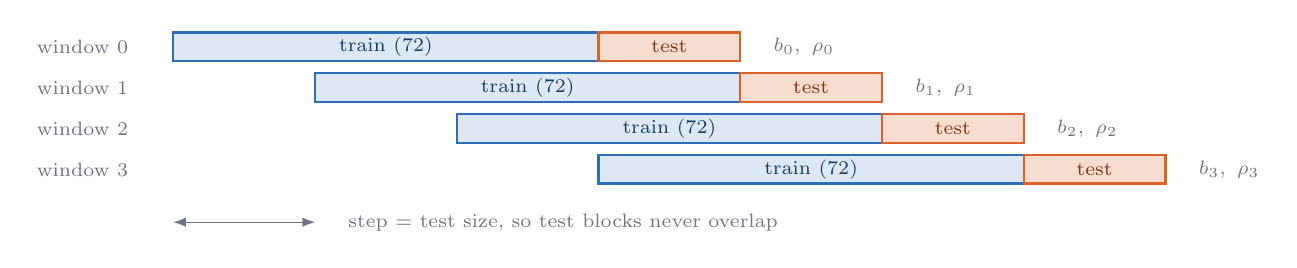
\begin{tikzpicture}[x=0.075cm, y=1cm, font=\footnotesize]
\foreach \i in {0,1,2,3} {
  \pgfmathsetmacro{\off}{24*\i}
  \pgfmathsetmacro{\yy}{-0.52*\i}
  \draw[fill=augBlue!16, draw=augBlue, thick] (\off,\yy) rectangle (\off+72,\yy+0.36);
  \node[font=\scriptsize, text=augBlue!55!black] at (\off+36,\yy+0.18) {train (72)};
  \draw[fill=augOrange!22, draw=augOrange, thick] (\off+72,\yy) rectangle (\off+96,\yy+0.36);
  \node[font=\scriptsize, text=augOrange!55!black] at (\off+84,\yy+0.18) {test};
  \node[anchor=east, font=\scriptsize, text=augGrey] at (-6,\yy+0.18) {window \i};
  \node[anchor=west, font=\scriptsize, text=augGrey] at (\off+100,\yy+0.18)
    {$b_{\i},\ \rho_{\i}$};
}
% step bracket
\draw[{Latex[length=1.6mm]}-{Latex[length=1.6mm]}, augGrey] (0,-2.05) -- (24,-2.05);
\node[anchor=west, font=\scriptsize, text=augGrey] at (28,-2.05)
  {step $=$ test size, so test blocks never overlap};
\end{tikzpicture}
\caption[Walk-forward evaluation windows]{Walk-forward evaluation in the C++ engine. Each window fits $b$ from its
own training-period order books and grid-searches responsiveness $\rho$ there,
then evaluates untouched on the test block. The step equals the test size, so no
observation is scored twice --- overlapping test windows would reuse data across
evaluations and make the results look more consistent than they are. The spread
of $b$ across windows is reported as a coefficient of variation, which
Table~\ref{tab:obs} suggests will be large.}
\label{fig:walkforward}
\end{figure}

The engine is deliberately file-in/file-out over JSON with no database or Redis
client. The numerical core is the part worth writing in C++; keeping the I/O
boundary at JSON means the binary is trivially testable and has no transport
dependencies to break. A separate benchmark target measures per-operation cost,
kept out of \code{ctest} because a benchmark has no pass/fail condition and
wiring one into CI makes the suite fail whenever a build agent is busy.

\section{Econometrics}
\label{sec:econ}

The question is whether $S(t)$ carries information about where $P(t)$ goes next,
beyond what $P$'s own history already implies. The vector autoregression is

\begin{equation}
P_t = \alpha_0 + \sum_{j=1}^{p} \alpha_j P_{t-j} + \sum_{j=1}^{p} \beta_j S_{t-j} + \epsilon_t,
\qquad H_0: \beta_1 = \cdots = \beta_p = 0.
\end{equation}

Four guards stand between a naive version of this test and a defensible answer,
and all four are enforced in code.

\paragraph{Logit transform.} $P_t \in [0,1]$ and $S_t \in [-1,1]$ are both
bounded. A market at $0.03$ cannot fall much further, so its innovations are
asymmetric and its level is near-certainly not stationary in the sense the VAR
requires. Both series are mapped through
$\tilde{x} = \ln\!\big(x/(1-x)\big)$ before fitting, with $S$ first mapped to
$(S+1)/2$ so it can share the transform. Lag order $p$ is chosen by AIC or BIC,
capped at $\min\!\big(12, \lfloor (n-2)/4 \rfloor\big)$ so the VAR is never fit
on fewer effective observations than it has coefficients.

\paragraph{Stationarity is tested, not assumed.} An Augmented Dickey--Fuller
result travels with every reported test, for both series. Granger causality
between two integrated series manufactures impressive $p$-values out of pure
spurious regression. The ADF null is a unit root, so a \emph{small} $p$-value is
evidence \emph{for} stationarity --- the opposite of the intuition most readers
carry into it, which is why the R implementation returns the result as a named
list rather than a bare number.

\paragraph{Alignment is a fixed convention, not a parameter.} Lead--lag results
are extremely sensitive to how the two series are joined. Post time is
\code{created\_at}, price time is bar close, both are resampled onto the same
regular grid by last-value-in-bar, and a value is carried across \emph{at most
one} empty bar. A loose \code{merge\_asof} tolerance --- as the Phase 1
prototype used, at two hours --- will pair a stale price with fresh sentiment
and produce a relationship that is an artifact of the join.

This convention is also where the deepest defect in the codebase was found. The
R implementation originally bucketed timestamps with \code{cut()}, which returns
a \emph{factor} whose levels are wall-clock strings carrying no timezone;
\code{as.POSIXct()} then reinterpreted each label in the session's local zone and
silently shifted every timestamp by the UTC offset, so the signal/price join
matched almost nothing. The covering test asserted only an upper bound on row
count, so it passed at zero rows. The fix is integer arithmetic on epoch
seconds, which is exact and zone-independent.

\paragraph{Multiple comparisons.} Running this test once per market across dozens
of markets at $p < 0.05$ produces roughly one false ``sentiment leads price''
finding per twenty by chance. A Benjamini--Hochberg FDR correction is applied
across the whole batch, and the \code{significant} field is defined off the
adjusted $p$-value \emph{only} --- it is \code{NA} until the correction runs, and
an uncorrected result reports as not significant, because in isolation it is not
yet an answer. The serving layer enforces the same discipline: the
\code{/granger} endpoint returns only the newest \code{run\_id}, since mixing
runs means mixing $p$-values corrected against different batches.

The reverse direction (\code{price\_to\_signal}) is a first-class option
throughout, because a signal that merely \emph{follows} price is the null result
this project should be able to report cleanly.

\subsection{Forecast calibration}

When a market resolves at time $T$ to outcome $O \in \{0,1\}$, accuracy is
scored by the Brier score $\text{BS} = \frac{1}{N}\sum_t (\hat{p}_t - O)^2$.

Note the $\hat{p}_t$, not $S(t)$. The signal ranges over $[-1,1]$ and is not a
probability; scored directly, a maximally bearish signal $S = -1$ against an
outcome of $0$ --- a \emph{correct} call --- would contribute $(-1-0)^2 = 1$,
the worst possible value. The signal is mapped into probability space first, and
which mapping was used is stored alongside every score, because scores computed
under different mappings are not comparable quantities. Two mappings exist:
\textbf{affine}, $\hat{p} = (S+1)/2$, assumption-free and always available; and
\textbf{Platt}, $\hat{p} = \sigma(a + bS)$, fit by Newton--Raphson on the
two-parameter logistic over resolved markets.

The Platt fit targets \emph{smoothed} labels following Platt's original
formulation, $y^{+} = (N^{+}+1)/(N^{+}+2)$ and $y^{-} = 1/(N^{-}+2)$. This is
not cosmetic. Augury will have a handful of resolved markets long before it has
many, and small samples are frequently linearly separable --- every market the
signal called bullish happened to resolve YES. Against raw $0/1$ labels the
maximum-likelihood solution for separable data is unbounded: Newton drives $b$
toward infinity, log loss toward zero, and the resulting ``calibrator'' reports
probabilities of exactly $1.0$. A model whose entire purpose is tempering
overconfidence would instead be manufacturing it. The reported loss is computed
against the true $0/1$ outcomes rather than the smoothed targets, since
smoothing is a fitting device and quoting the smoothed loss would flatter the
model. The fit refuses to run at all when every resolved market in the batch had
the same outcome, on the grounds that such a batch says nothing about where the
decision boundary sits.

\begin{figure}[htbp]
\centering
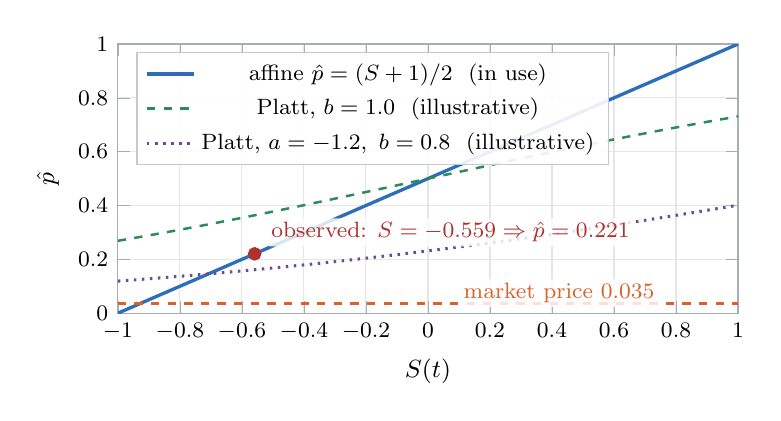
\begin{tikzpicture}
\begin{axis}[
  augbase, height=5.0cm,
  xlabel={$S(t)$}, ylabel={$\hat{p}$},
  xmin=-1, xmax=1, ymin=0, ymax=1,
  legend pos=north west,
]
\addplot[augBlue, line width=1.2pt, domain=-1:1, samples=2] {(x+1)/2};
\addlegendentry{affine $\hat{p}=(S+1)/2$ \ (in use)}
\addplot[augGreen, dashed, domain=-1:1, samples=120] {1/(1+exp(-(0 + 1.0*x)))};
\addlegendentry{Platt, $b=1.0$ \ (illustrative)}
\addplot[augPurple, dotted, line width=1.1pt, domain=-1:1, samples=120] {1/(1+exp(-(-1.2 + 0.8*x)))};
\addlegendentry{Platt, $a=-1.2,\ b=0.8$ \ (illustrative)}
% the observed point
\addplot[augRed, only marks, mark=*, mark size=2pt] coordinates {(-0.559,0.2205)};
\addplot[augOrange, dashed, line width=1pt] coordinates {(-1,0.035) (1,0.035)};
\node[annot, text=augRed, anchor=west] at (axis cs:-0.52,0.30) {observed: $S=-0.559 \Rightarrow \hat{p}=0.221$};
\node[annot, text=augOrange, anchor=west] at (axis cs:0.1,0.075) {market price $0.035$};
\end{axis}
\end{tikzpicture}
\caption[Affine versus Platt signal-to-probability mappings]{Mapping the signal into probability space. The affine map is a straight
line through $(0, 0.5)$ --- it asserts that a neutral signal means even odds,
which on a market trading at $0.035$ is badly wrong, and is the whole of the
$18.5$-point gap in Section~\ref{sec:worked}. A Platt fit is the mechanism for
correcting it, and the illustrative curves show the shape it would take: an
intercept $a<0$ shifts the whole map toward the base rate and a slope $b<1$
pulls in the extremes. \textbf{No fit exists yet}, because no tracked market has
resolved; these parameters are drawn to show the direction of the correction,
not measured.}
\label{fig:calibmap}
\end{figure}

Reported alone, the Brier score still answers the wrong question: a market that
traded at $0.02$ for a month and resolved NO yields a superb score for any
forecast that also said ``no''. The reported quantity is therefore the Brier
Skill Score against the market's own price at the same timestamps:

\begin{equation}
\text{BSS} = 1 - \frac{\text{BS}_{\text{signal}}}{\text{BS}_{\text{market}}}.
\end{equation}

$\text{BSS} > 0$ means the X-derived signal is better calibrated than the market
price itself --- the actual claim this project exists to support or refute.
$\text{BSS} \le 0$ is an equally useful result: it says the market is already
efficient with respect to this signal. Both branches are implemented, named, and
printed in plain language.

\section{Cross-Language Verification}
\label{sec:golden}

The same mathematics is implemented three times: in Python (the reference), in
C++ (the simulation engine), and in R (the analytics module). Independent
implementations of a formula agree only by luck unless something forces the
issue.

The forcing function is \code{schemas/testdata/golden\_vectors.json}, generated
from the Python reference by \code{python -m augury\_signal.golden} at a fixed
epoch so the file is byte-identical between runs. It holds 53 cases
(Table~\ref{tab:golden}), emitted at full float64 repr precision; the consuming
suites compare at $10^{-9}$, loose enough to absorb differences in summation
order and tight enough that a genuine formula divergence cannot hide.

\begin{table}[htbp]
\centering
\caption[Golden-vector inventory]{Golden-vector inventory. Each case fixes inputs and the expected output
of the Python reference.}
\label{tab:golden}
\small
\begin{tabular}{@{}llr l@{}}
\toprule
Group & Covers & Cases & Notable case \\
\midrule
\code{signal}                & $S(t)$ aggregation           & 7 & \code{extreme\_age}: weight underflows to $0$ \\
\code{lmsr.cost}             & $C(\mathbf{q})$, price vector & 6 & $q/b = 500$; $K = 4$ and $K = 3$ \\
\code{lmsr.trade}            & $C(\mathbf{q}+d\mathbf{q}) - C(\mathbf{q})$ & 3 & buys and sells \\
\code{lmsr.binary\_price}    & sigmoid identity              & 3 & $q_{\text{yes}} = -900$ \\
\code{lmsr.shares\_to\_move} & $b(\operatorname{logit} p' - \operatorname{logit} p)$ & 3 & $0.97 \to 0.03$ \\
\code{lmsr.b\_calibration}   & Eq.~\ref{eq:calib}            & 5 & the real Kalshi book; a crossed book \\
\code{adaptive\_decay}       & effective half-life           & 5 & floored at $t_{\min}$ \\
\code{calibration}           & affine, logit, sigmoid        & 21 & $\operatorname{logit}(0.001)$: boundary clamp \\
\midrule
\multicolumn{2}{@{}l}{\textbf{Total}} & \textbf{53} & \\
\bottomrule
\end{tabular}
\end{table}

The loop is closed. Each language asserts the subset it implements, to $10^{-9}$:
Python all 53 vectors, C++ the 20 LMSR vectors (43 Catch2 assertions across 5
cases), and R the 14 logit and affine vectors. The C++ engine now compiles and
runs, so that column is a measurement rather than a promise
(Section~\ref{sec:limits}). Regenerating after an intentional change to the
reference mathematics is expected to break the other suites, and that breakage
is the mechanism working rather than a nuisance to be routed around.

Two design details make this gate load-bearing rather than decorative. The
vectors are chosen to be hostile rather than representative --- a 30-day-old
post at a 30-minute half-life whose weight underflows to zero, a crossed book
that must fall back rather than raise, $q/b = 500$ in the cost function, and
logit inputs of $0.001$ and $0.999$ that exercise the boundary clamp instead of
diverging. And the C++ suite locates the file by walking up from the build
directory, so the gate cannot be accidentally skipped by a build layout change;
a missing file fails the suite rather than silently passing zero assertions.

\section{Serving Layer}
\label{sec:serving}

The Java service is a reactive Spring Boot gateway over the same schema, plus
the paper-trading ledger. Three decisions are worth recording.

\paragraph{Blocking work never touches the event loop.} Every JDBC call is
wrapped so that it runs on the bounded-elastic scheduler rather than the
reactor thread:
%
\begin{center}
\code{Mono.fromCallable(work).subscribeOn(Schedulers.boundedElastic())}
\end{center}
%
Blocking a Netty worker thread stalls every other request that thread is
multiplexing; with a small worker pool that is a service-wide outage rather
than one slow response.

\paragraph{SQL NULL is not zero.} \code{ResultSet.getDouble} returns $0.0$ for
SQL \code{NULL}, and for a price that is a meaningful and wrong value --- $0.0$
means ``certain NO'', not ``unknown''. Every optional numeric goes through a
\code{wasNull()}-checked accessor. The same principle governs the valuation
path: a position with no available mark returns a null price and an explicitly
incomplete valuation rather than an unrealised P\&L of zero, which would read as
``flat''.

\paragraph{Optional filters need explicit casts.} PostgreSQL infers a
parameter's type from how it is used, and a parameter appearing \emph{only}
inside \code{? IS NULL} gives it nothing to infer from; the server rejects the
statement with ``could not determine data type of parameter''. Every optional
filter is written \code{CAST(? AS text) IS NULL OR col = ?}. This was a shipped
defect: the unit tests mock the repository, so the SQL was never executed
against a server, and the failure appears only at runtime.

The paper-trading ledger holds no venue credentials of any kind, which is an
architectural boundary rather than an unfinished feature. Its sizing rule is
worth stating because it encodes the project's thesis directly: the target
position is proportional to the signal's \emph{edge over the market}
$\hat{p} - p_{\text{market}}$, not to the signal level. A signal saying ``80\%
likely'' is worth nothing when the market already says 80\%; it is informative
only when it disagrees. Sizing on the level alone would pile into consensus
positions and mistake agreement for insight.

\section{A Worked End-to-End Run}
\label{sec:worked}

The \code{slice} subcommand executes the entire chain in memory --- poll, ingest,
score, aggregate, simulate, analyse --- with no database and no billable API
calls. It was run twice against \code{kalshi:KXFEDDECISION-26SEP-C25}, six days
apart. The second run was not planned; it was executed to produce the figures in
this section, and what it found is more informative than what it was for.
Table~\ref{tab:slice} reports the first.

\begin{table}[htbp]
\centering
\caption[Vertical slice results, 28 July 2026]{Vertical slice, \code{kalshi:KXFEDDECISION-26SEP-C25}, 28 July 2026.
Prices and order book are live Kalshi data; posts are fixture replay.}
\label{tab:slice}
\small
\begin{tabular}{@{}ll@{}}
\toprule
Stage & Result \\
\midrule
Price history        & 278 hourly bars fetched \\
Order book           & bid $0.03 \times 93$, ask $0.04 \times 67{,}296$, spread $0.0100$ \\
Calibrated $b$       & $113{,}052$ (mean side; see Table~\ref{tab:depth}) \\
Posts                & 12, fixture replay, \code{source='fixture'} \\
Stance model         & \code{vader-3.3.2} (lexicon baseline) \\
$S(t)$ series        & 49 hourly points; latest $S = -0.559$, $\hat{p} = 0.221$ \\
Effective half-life  & 6.00 h (no surge trigger fired) \\
LMSR path            & $0.147 \to 0.220$ over 49 steps \\
Real market mid      & $0.035$ \quad (gap $+0.185$) \\
Strongest $|r|$      & $+0.658$ at lag $-3$\,h --- \emph{price leads} \\
Granger $S \to P$    & $F = 1.003$, $p = 0.463$, lag 7 (AIC), $n = 39$ \\
ADF $p$-values       & signal $0.144$ (unit root not rejected), price $0.025$ \\
Calibration          & market unresolved; Brier/BSS deferred \\
\bottomrule
\end{tabular}
\end{table}

What this run demonstrates and what it does not are different things, and the
tool says so itself: the report terminates with an explicit notice that posts
were replayed and the numbers are not evidence about the real relationship
between X and this market.

Read as an instrument check, several things are working correctly. The
cross-correlation peak sits at lag $-3$\,h with the interpretation label
\emph{price leads} --- the direction that falsifies the project's hypothesis,
reported as prominently as the direction that would confirm it. The Granger test
does not reject at any conventional level, and the report immediately annotates
that this is an uncorrected $p$-value which requires Benjamini--Hochberg
adjustment across every market before it means anything. And the ADF test fails
to reject a unit root in the signal series at $p = 0.144$ --- which is not
evidence that the series \emph{is} integrated, but is exactly the condition
under which the $F$ statistic printed two lines above it should not be trusted.
The guard fired and said so rather than being silently satisfied.

Two things visible here are genuinely problematic and worth naming. The
simulated LMSR price ends at $0.220$ against a real market mid of $0.035$, a gap
of $18.5$ probability points. That gap is not evidence of predictive power; it
is the affine mapping $\hat{p} = (S+1)/2$ doing exactly what
Section~\ref{sec:econ} predicts it will do on an out-of-the-money market. A
moderately bearish lexicon signal of $S = -0.559$ maps to $\hat{p} = 0.221$,
roughly six times the market's own price, because the affine map's implicit
claim that $S = 0$ means $50/50$ is a strong and here plainly false
assumption. This is precisely the case Platt
calibration exists to correct, and it cannot be fit until markets resolve. The
second is that this run used the VADER lexicon rather than the NLI model, so the
stance scores are sentiment, not stance, and the sign is untrustworthy on exactly
the phrasing Section~\ref{sec:stance} describes.

\subsection{A second observation, six days later}
\label{sec:obs2}

Re-running the identical command on 3 August produced a materially different
picture (Table~\ref{tab:obs}). The market had drifted from $0.035$ to $0.015$ and
then stopped moving; the book had thickened by three orders of magnitude on both
sides. Nothing in the code changed. Everything downstream did.

\begin{table}[htbp]
\centering
\caption[The same market, six days apart]{The same command, the same market, six days apart. Only the venue data
differs. The fixture-replayed signal is deterministic and reproduces exactly,
which isolates every change below to the market side.}
\label{tab:obs}
\small
\begin{tabular}{@{}lrr@{}}
\toprule
& 28 July 2026 & 3 August 2026 \\
\midrule
Market mid                & $0.0350$ & $0.0150$ \\
Best bid $\times$ depth   & $0.03 \times 93$ & $0.01 \times 98{,}329$ \\
Best ask $\times$ depth   & $0.04 \times 67{,}296$ & $0.02 \times 858{,}548$ \\
Logit width               & $0.2980$ & $0.7033$ \\
\midrule
$b$ (bid side)            & $312$ & $139{,}811$ \\
$b$ (mean)                & $113{,}052$ & $680{,}277$ \\
$b$ (ask side)            & $225{,}792$ & $1{,}000{,}000$\rlap{$^{\dagger}$} \\
\midrule
Latest $S(t)$             & $-0.559$ & $-0.559$ \\
LMSR path end             & $0.220$ & $0.220$ \\
Distinct prices in window & $\ge 3$ & \textbf{2} \\
Granger $S \to P$         & $F=1.003$, $p=0.463$ & \textbf{refused (degenerate)} \\
\bottomrule
\end{tabular}

\vspace{2pt}
{\footnotesize $^{\dagger}$ clamped at \code{B\_MAX}; the uncapped value is
$1{,}220{,}743$. The 28 July distinct-price count is recorded only as
$\ge 3$, which is what the guard passing establishes.}
\end{table}

Three things follow, and they are the most useful empirical results in this
paper.

\paragraph{The liquidity calibration is not stable.} $b$ moved by a factor of six
on the mean side, and on the ask side it left the representable band entirely and
hit the \code{B\_MAX} clamp of $10^{6}$. Section~\ref{sec:lmsr} argued from
Table~\ref{tab:depth} that the choice of \emph{side} was worth $723\times$;
Table~\ref{tab:obs} adds that the choice of \emph{day} is worth another $6\times$
on top of it. The C++ backtester's coefficient-of-variation warning was written
against exactly this failure, and two observations are already enough to trip it.
Figure~\ref{fig:book} shows why: on this market the book is not merely lopsided,
it is lopsided by a different amount every time it is sampled.

\paragraph{The degeneracy guard fired, and it was right to.} With the market
pinned at $0.015$ for the whole window, the Granger path refused to run and
printed \emph{``market price is nearly constant over this window --- the test is
degenerate''} instead of a $p$-value. This is the behaviour
Section~\ref{sec:econ} was designed for, observed rather than asserted:
the honest output on this data is no number at all.

\paragraph{But the cross-correlation did not refuse, and it should have.} This is
a defect, and unlike those in Table~\ref{tab:defects} it is a runtime one. Both
guards test how many distinct prices the window holds, but they disagree on this
data:

\begin{center}
\small
\begin{tabular}{@{}lll@{}}
\toprule
Guard & Condition & Outcome \\
\midrule
Cross-correlation & \code{len(set(prices)) < 2} & does \emph{not} fire --- CCF runs \\
Granger           & \code{len(set(prices)) < 3} & fires --- test correctly skipped \\
\bottomrule
\end{tabular}
\end{center}

The window contains two distinct \code{float} values, $0.015$ and
$0.01500000000000001$, which differ by $1.04 \times 10^{-17}$ --- six units in
the last place. They are not two prices. They are one price and a rounding
artifact, produced because the YES ask is derived as $1 - 0.98$, which is not
representable in binary64. Set cardinality cannot tell the difference, so the
looser guard sees ``two distinct values'', concludes the market moved, and
computes a cross-correlation of $S(t)$ against floating-point noise. The
resulting table (Figure~\ref{fig:ccf}, right) reports coefficients rising
smoothly to $-0.398$ at lag $+6$ --- a clean, entirely spurious signal-leads-price
gradient, which is precisely the finding this project is built not to produce.

The fix is to test the range against a tolerance rather than the cardinality of a
float set --- \code{ptp(prices) < 1e-9} --- and to apply the same threshold in
both places, since there is no reason for two guards over the same question to
disagree. It is worth noting how narrowly this was caught: had the market moved
one tick more, the Granger guard would have passed too, and the run would have
reported a $p$-value computed on noise.

\begin{figure}[htbp]
\centering
\begin{tikzpicture}
\begin{axis}[
  augbase, height=5.4cm,
  xlabel={Hours since first signal point}, ylabel={Probability},
  xmin=0, xmax=47, ymin=0, ymax=0.85,
  legend pos=north east, legend columns=1,
]
\addplot[augBlue, line width=1.1pt] table[x=hour, y=p_hat, col sep=comma] {data/series.csv};
\addlegendentry{$\hat{p} = (S(t)+1)/2$ \ (signal)}
\addplot[augPurple, dashed, line width=1pt] table[x=hour, y=sim, col sep=comma] {data/series.csv};
\addlegendentry{LMSR simulated price}
\addplot[augOrange, line width=1.3pt] table[x=hour, y=market, col sep=comma] {data/series.csv};
\addlegendentry{real Kalshi mid}
\node[annot, text=augOrange, anchor=west] at (axis cs:14,0.075)
  {real market: flat at $0.015$ for all 48 bars};
\end{axis}
\end{tikzpicture}
\caption[Signal, simulated price, and real market, 3 August run]{The 3 August run, plotted from \code{paper/data/series.csv}. The signal
moves across most of the unit interval and the LMSR integrates it; the real
market does not move at all. The orange line is not a plotting artifact --- it is
the entire basis on which the cross-correlation in Figure~\ref{fig:ccf} was
computed.}
\label{fig:series}
\end{figure}

\begin{figure}[htbp]
\centering
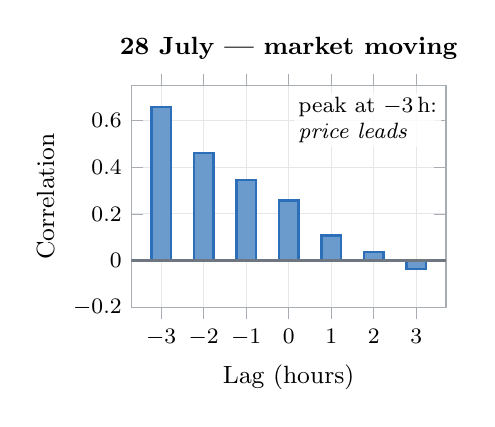
\begin{tikzpicture}
\begin{axis}[
  augsmall, title={28 July --- market moving},
  xlabel={Lag (hours)}, ylabel={Correlation},
  xmin=-3.7, xmax=3.7, ymin=-0.2, ymax=0.75,
  xtick={-3,-2,-1,0,1,2,3},
  ybar, bar width=7pt,
]
\addplot[fill=augBlue!70, draw=augBlue] coordinates
  {(-3,0.6576) (-2,0.4605) (-1,0.3452) (0,0.2569) (1,0.1068) (2,0.0374) (3,-0.0353)};
\addplot[augGrey, sharp plot, update limits=false] coordinates {(-3.7,0) (3.7,0)};
\node[annot, anchor=north east] at (axis cs:3.6,0.72) {peak at $-3$\,h:\\ \emph{price leads}};
\end{axis}
\end{tikzpicture}%
\hfill
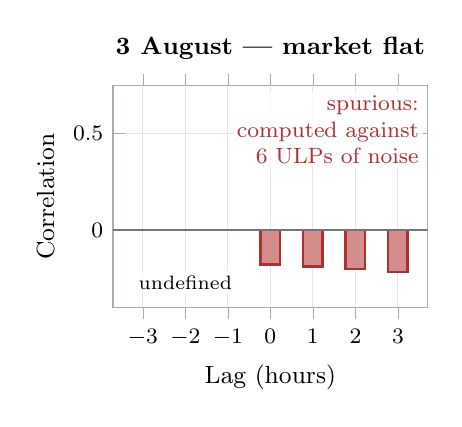
\begin{tikzpicture}
\begin{axis}[
  augsmall, title={3 August --- market flat},
  xlabel={Lag (hours)}, ylabel={Correlation},
  xmin=-3.7, xmax=3.7, ymin=-0.4, ymax=0.75,
  xtick={-3,-2,-1,0,1,2,3},
  ybar, bar width=7pt,
]
\addplot[fill=augRed!55, draw=augRed] coordinates
  {(0,-0.1770) (1,-0.1885) (2,-0.2016) (3,-0.2168)};
\addplot[augGrey, sharp plot, update limits=false] coordinates {(-3.7,0) (3.7,0)};
\node[annot, text=augRed, anchor=north east, align=right] at (axis cs:3.6,0.72)
  {spurious:\\ computed against\\ 6 ULPs of noise};
\node[annot, anchor=south, font=\scriptsize] at (axis cs:-2,-0.33) {undefined};
\end{axis}
\end{tikzpicture}
\caption[Cross-correlation, both observations]{Cross-correlation of $S(t)$ against price, both runs, lags $-3$ to $+3$.
Left: a real gradient peaking on the \emph{price-leads} side, the direction that
falsifies the hypothesis. Right: the same computation on a market that never
moved, which the guard failed to reject. The right panel is not a weaker version
of the left one --- it is a measurement of nothing, and it looks more like a
finding than the real data does.}
\label{fig:ccf}
\end{figure}

\begin{figure}[htbp]
\centering
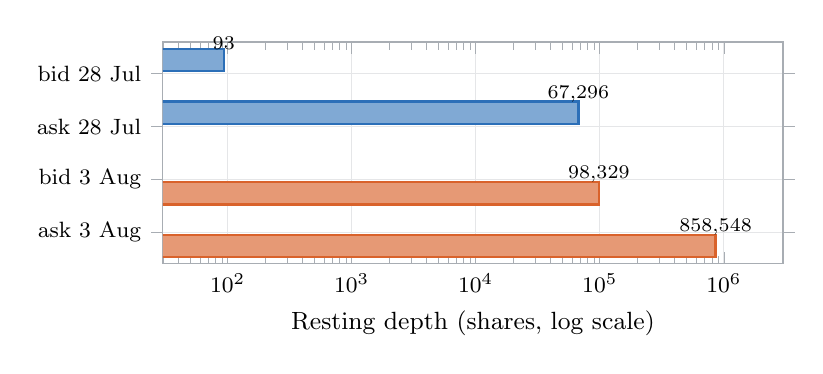
\begin{tikzpicture}
\begin{semilogxaxis}[
  augbase, height=4.4cm,
  xlabel={Resting depth (shares, log scale)},
  xmin=30, xmax=3e6,
  ytick={1,2,3,4}, yticklabels={ask 3 Aug, bid 3 Aug, ask 28 Jul, bid 28 Jul},
  ymin=0.4, ymax=4.6,
  xbar, bar width=8pt,
  point meta=explicit symbolic,
  nodes near coords, every node near coord/.append style={font=\scriptsize},
]
\addplot[fill=augOrange!65, draw=augOrange] coordinates {(858548,1) [858,548] (98329,2) [98,329]};
\addplot[fill=augBlue!60, draw=augBlue] coordinates {(67296,3) [67,296] (93,4) [93]};
\end{semilogxaxis}
\end{tikzpicture}
\caption[Resting order-book depth, both observations]{Resting depth on each side of the book, both observations, on a log
axis. On 28 July the two sides differed by $723\times$; on 3 August by
$8.7\times$, with both sides three orders of magnitude thicker. Equation~\ref{eq:calib}
turns each of these bars directly into a liquidity parameter, which is why $b$ is
not reproducible across days.}
\label{fig:book}
\end{figure}
\section{Defects Found by Review}

A full correctness review was run over the codebase. Table~\ref{tab:defects}
records what it found. Each entry is a class of bug the existing tests could not
have caught, which is the property that makes them worth recording rather than
silently fixing.

\begin{table}[htbp]
\centering
\caption[Defects found by review]{Defects found by review, and why the test suite missed each.}
\label{tab:defects}
\small
\begin{tabular}{@{}p{0.20\textwidth}p{0.36\textwidth}p{0.34\textwidth}@{}}
\toprule
Location & Defect & Why tests missed it \\
\midrule
R \code{align\_on\_grid} &
\code{cut()} dropped the timezone, shifting every timestamp by the local UTC
offset; the join matched almost nothing. &
The covering test asserted only an upper bound on row count, so it passed at
zero rows. \\[2pt]
Java \code{AuguryRepository} &
Optional filters used a bare \code{? IS NULL}, which PostgreSQL rejects with
``could not determine data type of parameter''. &
Unit tests mock the repository, so the SQL was never sent to a server. \\[2pt]
Rust \code{ReadBudget::}\allowbreak\code{reserve} &
The \code{ON CONFLICT} ceiling guard does not fire on the first insert of a UTC
day, so one request larger than the whole daily budget was allowed through. &
The path requires a live database and an empty budget table; integration tests
skip without \code{DATABASE\_URL}. \\[2pt]
C++ engine &
Five missing standard headers (\code{<cstdint>}, \code{<limits>},
\code{<string>}, \code{<utility>}, \code{<stdexcept>}). &
Found by inspection before a compiler was available. With the headers in place the
engine now compiles clean and its 26 Catch2 cases pass
(Section~\ref{sec:limits}). \\
\bottomrule
\end{tabular}
\end{table}

\subsection{A fifth defect, recorded as fixed but still present}

The review recorded a fifth item --- that Python's \code{simulate\_lmsr}
``recalibrated $b$ to the same constant every step, making per-step liquidity
tracking a no-op, and left a dead local behind'' --- and marked it resolved. It
is not resolved, and the distinction matters because the function's own
docstring makes a claim the implementation does not support.

The docstring states that ``$b$ is re-calibrated at each step from the most
recent book snapshot, so the synthetic market's sensitivity tracks the real
market's liquidity instead of being a constant chosen to make the output look
good.'' In the implementation, $b$ is computed once from a single book snapshot
before the loop begins, and the in-loop call is \code{market.recalibrate(b)}
with that same unchanged value.

That call is a no-op, and the proof takes two steps. By the invariance property
of Section~\ref{sec:lmsr}, recalibration rescales the share imbalance by
$b_{\text{new}}/b_{\text{old}}$ to hold
$\operatorname{logit}(p) = (q_{\text{yes}} - q_{\text{no}})/b$ fixed; with $b$
unchanged that ratio is exactly $1$. The method then canonicalises the state by
assigning the whole imbalance to the YES leg, which is \emph{not} in general an
identity --- but along this code path it is, because every mutation of the
market goes through \code{buy\_yes}, which touches only $q_{\text{yes}}$, so
$q_{\text{no}}$ is identically zero from construction onward. Both steps are
therefore identities, and the call cannot change any field of the market state.
The dead local likewise survives: it is now explicitly discarded with
\code{del ordered\_prices} at the end of the function, which silences the linter
without removing the dead computation.

There is a deeper reason the docstring cannot be satisfied as written. The price
polling step appends exactly \emph{one} order-book snapshot per cycle --- history
comes from candles, which carry bid and ask but no depth --- so there is no
per-step book history to calibrate against even in principle. The correct
version of this behaviour already exists in the C++ backtester, which calibrates
$b$ per walk-forward window from that window's own training-period books and
holds it fixed through the test period. Bringing the Python path in line means
either persisting a depth series or restating the docstring to describe what the
data supports. Both are legitimate; silently disagreeing with the docstring is
not, which is why it is reported here rather than quietly patched.

\section{Verification Status and Limitations}
\label{sec:limits}

\begin{table}[htbp]
\centering
\caption[Test inventory]{Test inventory. Every suite has now been executed; no row is a
projection.}
\label{tab:tests}
\small
\begin{tabular}{@{}llll@{}}
\toprule
Suite & Framework & Count & Status \\
\midrule
\code{augury-signal} & pytest   & 139 tests & \textbf{pass} (1.3 s, ruff clean) \\
\code{augury-analytics} & testthat & 55 expectations & \textbf{pass} \\
\code{augury-api}    & JUnit    & 9 tests   & \textbf{pass} (JDK 25; also JDK 21) \\
\code{augury-ingest} & cargo    & 42 tests  & \textbf{pass} (GNU target) \\
\code{augury-engine} & Catch2   & 26 cases  & \textbf{pass} (97 assertions) \\
\bottomrule
\end{tabular}
\end{table}

Table~\ref{tab:tests} is the honest accounting, and it has changed. An earlier
version of this section reported that two of the five services had never been
compiled, and treated that as a standing limitation: uncompiled code is
unverified code. Both have since been built and run, and the table now records
measurements rather than intentions.

The correction worth recording is the diagnosis, not just the outcome. Rust
failures had been attributed to Windows Smart App Control blocking the unsigned
\code{build.rs} executables Cargo compiles and runs. Smart App Control remains
\emph{Enforced} on the same machine, and both services nonetheless build and pass.
The operative blocker was narrower and shared: no C++ toolchain was installed, and
Rust's default \code{x86\_64-pc-windows-msvc} target links through MSVC's
\code{link.exe}, so cargo failed at link time rather than at the build script.
Building Rust against \code{x86\_64-pc-windows-gnu} with a MinGW-w64 toolchain
clears it without administrative rights, and the same toolchain builds the C++
engine. No source change was required in either service.

That the C++ engine compiled unmodified is itself weak evidence: the five missing
standard headers recorded in the correctness review were found by inspection
before any compiler existed to find them, and no further compilation defects
surfaced. The Rust build emitted nine dead-code warnings and no errors.

Beyond that:

\begin{itemize}\itemsep3pt
\item \textbf{No lead--lag result exists.} A Granger test on a handful of hourly
      bars proves nothing. The ingester must run for days to weeks per market
      before any finding is worth reporting, and the Platt calibration cannot be
      fit until several markets have actually resolved with both outcomes
      represented.
\item \textbf{The stance path needs a real checkpoint in production.} The
      default is NLI-tuned, which makes zero-shot stance detection work without a
      labelled corpus, but a fine-tune on prediction-market stance data would
      very likely beat it --- and the run in Section~\ref{sec:worked} used the
      lexicon baseline, not the NLI model.
\item \textbf{Test coverage is uneven.} The pure-mathematical core is thoroughly
      covered and cross-validated; the database layer, Redis bus, and pipeline
      orchestration are not, the Java tests cover ledger arithmetic rather than
      the controllers, and there is no cross-service integration suite. Two of
      the four defects in Table~\ref{tab:defects} live in exactly those gaps.
\item \textbf{Liquidity controls are specified but not wired in.} Depth and
      spread are collected and stored, and \code{granger\_results.liquidity\_control}
      records whether a run used them --- it is currently always false. Without
      them, ``sentiment leads price'' can be an artifact of when the book
      happened to be thin.
\item \textbf{The LSH banding fix in Section~\ref{sec:ingest} is analysed, not
      applied.} Changing it invalidates stored bucket keys, so it requires a
      migration rather than a constant edit.
\item \textbf{The degeneracy guards are inconsistent and both are unapplied
      fixes.} Section~\ref{sec:obs2} shows the cross-correlation and Granger
      paths disagreeing on whether a window is degenerate, because one tests
      \code{len(set(prices))} against 2 and the other against 3. Both should
      test the range against a tolerance. Until they do, any cross-correlation
      reported on a near-static market is untrustworthy.
\end{itemize}

\section{Conclusion}

Augury is an instrument, and this paper is its calibration report. The
mathematics it implements --- a decay-weighted stance aggregate, a
depth-calibrated LMSR market maker, a guarded Granger test, and a
market-referenced Brier skill score --- is not individually novel. What the
system contributes is the discipline around it: three independent
implementations held to one shared set of deliberately hostile golden vectors,
two of them currently executed against it; statistical guards enforced in code
rather than in the analyst's memory; and an evaluation path on which the answer ``the market is already
efficient with respect to this signal'' is as easy to reach and as clearly
printed as its opposite.

The analysis in this paper produced three corrections to the system's own
claims. The float64 underflow threshold for the decay kernel is
$\lambda \Delta t > 745$, not $233$, so the documented danger zone was off by a
factor of three in the conservative direction. The shipped LSH band
configuration achieves $20.4\%$ retrieval at its own declared duplicate
threshold, which the asymmetric cost structure of a pre-filter says should be
closer to $95\%$; the fix is a repartitioning of an existing signature, not new
machinery. And the per-step liquidity recalibration described in the simulation
docstring is a provable no-op as implemented, for the structural reason that the
pipeline stores only one book snapshot per cycle. None of the three was found by
the test suite, and none could have been: two are incorrect \emph{claims} about
correct code, which no assertion is written to catch, and the third is a
function that satisfies every test while contradicting its own docstring. Two
surfaced from working the arithmetic out on paper and checking it against the
source; the third from reading the implementation against the behaviour it
advertises.

The fourth was different, and it is the one that most justifies the exercise.
Running the same command six days later on a market that had gone flat produced
a cross-correlation table with a smooth gradient to $-0.398$ on the
signal-leads-price side --- computed entirely against six units in the last
place of floating-point rounding noise, because the guard tested the cardinality
of a float set rather than the range of the series. The Granger path, testing
the same question with a stricter threshold, refused correctly. Two guards over
one question disagreed, and the looser one produced exactly the artifact this
project exists not to produce. No amount of reasoning about the code surfaced
that; it took running it on a day when the market had stopped moving. An
instrument that is only ever reasoned about is not yet calibrated.

The generalisable point is the one the null result makes available. On a
question where the prior should be that the effect does not exist, an apparatus
that cannot report its absence is not measuring anything. The guards documented
here --- FDR correction before significance is defined, a random-walk baseline on
every backtest window, a market-referenced skill score, and a
$b$-stability statistic that invalidates its own MSE figures when it drifts ---
exist so that when the ingester has run long enough to produce an answer, the
answer will be worth the wait, in whichever direction it falls.

\appendix

\section{The slice report, verbatim}
\label{app:slice}

Output of \code{python -m augury\_signal.cli slice --market KXFEDDECISION-26SEP-C25}
on 3 August 2026, unedited. Kalshi price and book data are live; posts are
fixture replay. This is the run tabulated in Table~\ref{tab:obs} and plotted in
Figures~\ref{fig:series}--\ref{fig:book}.

\begin{lstlisting}[basicstyle=\ttfamily\scriptsize]
====================================================================
AUGURY VERTICAL SLICE -- kalshi:KXFEDDECISION-26SEP-C25
====================================================================
  Will the Federal Reserve Cut rates by 25bps at their September 2026 meeting?
  target: The Federal Reserve will cut interest rates by 25 basis points at its September 2026 meeting.
  status: open

-- market data ---------------------------------------------------
  price bars fetched   : 277
  book                 : bid 0.01 / ask 0.020000000000000018  spread 0.0100
  depth (bid/ask)      : 98329.33 / 858548.26
  LMSR b (from depth)  : 680,277.41

-- social signal -------------------------------------------------
  post source          : FIXTURE REPLAY (no live X reads, no cost)
  posts                : 12
  stance model         : vader-3.3.2
  mean raw stance      : +0.0907
  S(t) points          : 48
  latest S(t)          : -0.5589  (p_hat 0.2205, 11 posts, half-life 6.00h)

-- synthetic LMSR market -----------------------------------------
  sim ticks            : 48
  sim price            : 0.0890 -> 0.2218
  real market mid      : 0.0150  (gap +0.2068)

-- lead-lag ------------------------------------------------------
  strongest |r|        : -0.3981 at lag +6h (signal leads, n=33)
    lag +0h  r = -0.1770  (contemporaneous)
    lag +1h  r = -0.1885  (signal leads)
    lag +2h  r = -0.2016  (signal leads)
    lag +3h  r = -0.2168  (signal leads)
  Granger              : market price is nearly constant over this window -- the test is degenerate

-- calibration ---------------------------------------------------
  market has not resolved yet -- Brier/BSS deferred to the watcher

====================================================================
Posts were replayed from fixtures. These numbers exercise the pipeline;
they are not evidence about the real relationship between X and this market.
====================================================================
\end{lstlisting}

Two lines are worth reading against each other. The Granger block refuses to
report a number and says why. Four lines above it, the cross-correlation block
reports a monotone gradient to $-0.398$ labelled \emph{signal leads} --- on the
same data, from the same window, with no such warning. That contrast is the
defect of Section~\ref{sec:obs2} as the tool actually prints it.

\clearpage
\phantomsection
\addcontentsline{toc}{section}{References}
\begin{thebibliography}{9}

\bibitem{hanson}
Hanson, R. (2003). Combinatorial information market design.
\emph{Information Systems Frontiers}, 5(1), 107--119.

\bibitem{hanson2007}
Hanson, R. (2007). Logarithmic market scoring rules for modular combinatorial
information aggregation. \emph{Journal of Prediction Markets}, 1(1), 3--15.

\bibitem{granger}
Granger, C. W. J. (1969). Investigating causal relations by econometric models
and cross-spectral methods. \emph{Econometrica}, 37(3), 424--438.

\bibitem{bh}
Benjamini, Y., \& Hochberg, Y. (1995). Controlling the false discovery rate: a
practical and powerful approach to multiple testing. \emph{Journal of the Royal
Statistical Society, Series B}, 57(1), 289--300.

\bibitem{brier}
Brier, G. W. (1950). Verification of forecasts expressed in terms of
probability. \emph{Monthly Weather Review}, 78(1), 1--3.

\bibitem{platt}
Platt, J. (1999). Probabilistic outputs for support vector machines and
comparisons to regularized likelihood methods. In \emph{Advances in Large Margin
Classifiers}, MIT Press, 61--74.

\bibitem{broder}
Broder, A. Z. (1997). On the resemblance and containment of documents. In
\emph{Proceedings of the Compression and Complexity of Sequences}, 21--29.

\bibitem{mmds}
Leskovec, J., Rajaraman, A., \& Ullman, J. D. (2020).
\emph{Mining of Massive Datasets}, 3rd ed., Ch. 3: Finding similar items.
Cambridge University Press.

\bibitem{deberta}
He, P., Gao, J., \& Chen, W. (2023). DeBERTaV3: Improving DeBERTa using
ELECTRA-style pre-training with gradient-disentangled embedding sharing.
\emph{ICLR 2023}.

\bibitem{yin}
Yin, W., Hay, J., \& Roth, D. (2019). Benchmarking zero-shot text
classification: datasets, evaluation and entailment approach.
\emph{EMNLP-IJCNLP 2019}, 3914--3923.

\bibitem{dickeyfuller}
Said, S. E., \& Dickey, D. A. (1984). Testing for unit roots in
autoregressive-moving average models of unknown order. \emph{Biometrika}, 71(3),
599--607.

\end{thebibliography}

\end{document}
